% Clase umemoria en inglés (si se cambia el idioma, borrar el archivo .aux)
\documentclass[english]{umemoria}

% ------------------------------------------------------------------------------
% PORTADA
% TODO: revisar los datos de la portada (comisión, auspicio).
% ------------------------------------------------------------------------------
\depto{Departamento de Ciencias de la Computación}
\author{Cristián Carrión Saldivia}
\title{Design and implementation of an Executable Specification for PISA}

% doble titulación: tesis de magíster + memoria de ingeniería
\tesis{Magíster en Ciencias de la Computación}
\memoria{Ingeniero Civil en Computación}

\guia{Éric Tanter}
\coguia{Joel Fuentes}

%\comision{Nombre Uno,Nombre Dos} % TODO: comisión pendiente

%\auspicio{Nombre Institución} % incluir en caso de recibir financiamiento

% tiene que ser el año en que se da el examen de grado (defensa)
%\anho{2026}

% ------------------------------------------------------------------------------
% PAQUETES
% ------------------------------------------------------------------------------
\usepackage[T1]{fontenc}
\usepackage{lmodern}
\usepackage[dvipsnames]{xcolor}
\usepackage{array}
\usepackage{booktabs}
\usepackage[numbers,sort&compress]{natbib}
\usepackage{lipsum} % solo para el texto provisorio de la portada

% Bibliografía en el índice con el número de página de su inicio y con su
% propio encabezado (la clase la agrega al índice después de imprimirla)
\let\bibliography\oldbib
\renewcommand{\bibsection}{%
	\chapter*{\bibname}%
	\addcontentsline{toc}{chapter}{\protect\numberline{}\bibname}%
	\markboth{\MakeUppercase\bibname}{\MakeUppercase\bibname}}

% ------------------------------------------------------------------------------
% CÓDIGO FUENTE
% ------------------------------------------------------------------------------
\definecolor{dkgray}{RGB}{90, 90, 90}
\definecolor{dkgreen}{RGB}{0, 150, 0}
\definecolor{lgray}{RGB}{240, 240, 240}
\definecolor{mauve}{RGB}{150, 0, 210}

\lstset{
	aboveskip=0.75em,
	backgroundcolor=\color{lgray},
	basicstyle={\small\ttfamily},
	belowskip=0.95em,
	breaklines=true,
	columns=fullflexible,
	commentstyle=\color{dkgreen}\upshape,
	frame=ltb,
	framerule=0pt,
	keepspaces=true,
	keywordstyle=\color{blue},
	numbers=left,
	numbersep=6pt,
	numberstyle=\tiny\color{dkgray},
	postbreak=\mbox{$\hookrightarrow$\space},
	showstringspaces=false,
	stringstyle=\color{mauve},
	tabsize=3
}

% Definición del lenguaje ASL (Arm Architecture Specification Language) para listings
\lstdefinelanguage{ASL}{
	morekeywords={
		var,let,constant,func,getter,setter,procedure,begin,end,
		if,then,else,elsif,for,to,downto,do,while,repeat,until,
		case,when,otherwise,return,array,of,type,record,enumeration,
		integer,boolean,bits,bit,UNKNOWN,UNPREDICTABLE,SEE
	},
	sensitive=true,
	morecomment=[l]{//},
	morestring=[b]"
}

% Nota TODO visible en el pdf: \todo{texto}
\newcommand{\todo}[1]{%
	\par\noindent\fcolorbox{red}{red!8}{\parbox{\dimexpr\linewidth-2\fboxsep-2\fboxrule\relax}{%
		\textbf{\textcolor{red}{TODO:}} #1}}\par}

\begin{document}

\frontmatter
\maketitle

% TODO: dedicatoria y agradecimientos son provisorios.
% Una tesis en inglés lleva el resumen en ambos idiomas.
\begin{resumen}
La mayoría de las ISA de GPU se especifican solo en prosa. Una
especificación en prosa no puede ejecutarse por sí sola, de manera que
cada herramienta construida sobre ella, ya sea un compilador, un
simulador o una suite de tests, opera según su propia interpretación
del texto, y cualquier interpretación puede estar equivocada. Una
especificación ejecutable reemplaza esas múltiples interpretaciones
por una sola. Se lee como documentación y se ejecuta para producir el
comportamiento que describe. Esta tesis desarrolla una especificación
ejecutable de PISA, la ISA virtual que Intel publicó para sus GPU. La
especificación está escrita en ASL, el Architecture Specification
Language de Arm.

La especificación cubre un subconjunto de PISA que modela la ejecución
a nivel de subgrupo. Con ese subconjunto, un kernel puede intercambiar
datos con el host, realizar aritmética de enteros, comunicar valores
entre lanes y ejecutar branches. PISA no define cómo avanzan los lanes
de un subgrupo ni cómo reconvergen, por lo que la especificación lo
define. Los lanes se ejecutan en lockstep, y los lanes divergentes
reconvergen mediante una regla stackless, que depende únicamente de
los program counters de cada lane. Un parser traduce los kernels de
PISA a ASL, y una host library expone la especificación compilada a
través de la interfaz de OpenCL, de modo que un kernel compilado desde
OpenCL corre en ella sin modificaciones.

La especificación se comprueba con una suite de tests. Esta incluye
smoke tests que cubren cada instrucción del subconjunto contra el
documento de PISA, y kernel tests compilados desde OpenCL que ponen a
prueba la divergencia y las operaciones entre lanes. La suite
encontró, además, errores en los ejemplos del documento de PISA. Hasta
donde sabemos, esta es la única especificación ejecutable de PISA.
\end{resumen}

\begin{abstract}
Most GPU ISA specifications exist only in prose. A prose
specification cannot run by itself, so each tool built on it, a
compiler, a simulator, a test suite, works from its own interpretation of the text, and an
interpretation can be mistaken. An executable specification replaces
those separate interpretations with a single one that runs. It reads as
documentation and runs to produce the behavior it describes.
This thesis develops an executable specification of PISA, the virtual 
instruction set Intel has published for its GPUs. The specification is 
written in ASL, Arm's Architecture Specification Language.

The specification covers a subset of PISA that models execution at the
sub-group level. It can exchange data with the host, perform integer arithmetic, 
communicate across lanes, and branch. PISA does not define how the
lanes of a sub-group advance or how they reconverge, so the
specification defines it. Lanes
execute in lockstep, and divergent lanes reconverge by a stackless rule
driven by the per-lane program counters alone. A parser translates PISA
kernels into ASL, and a host library exposes the compiled specification
through the OpenCL interface, so that kernels compiled from OpenCL run
on it without change.

The specification is checked against a test suite. It includes smoke tests that
cover every instruction of the subset against the PISA document, and
kernel tests compiled from OpenCL that exercise divergence and
cross-lane operations. The suite also found errors in the examples of
the PISA document. To our knowledge, this is the only executable
specification of PISA.
\end{abstract}

\begin{dedicatoria}
Una frase de dedicatoria, \\
pueden ser dos líneas.
\end{dedicatoria}

\begin{thanks}
\lipsum[1]
\end{thanks}

\tableofcontents
\listoftables
\listoffigures

\mainmatter

% ------------------------------------------------------------------------------
% CAPÍTULOS
% Cada capítulo vive en chapters/. El material antiguo que no pertenece a
% ningún capítulo vigente está en chapters/draft.tex, que NO se compila.
% ------------------------------------------------------------------------------
\chapter{Introduction}
\label{chap:introduction}

\section{Motivation}

The GPU industry has grown significantly in the last decade, driven by
applications far beyond its traditional purpose in graphics rendering.
GPUs are now essential in machine learning, one of today's fastest-growing
industries, as well as in scientific computing, data analytics, and
autonomous systems. As GPU architectures have evolved to meet these
demands, they have become more complex, incorporating sophisticated
memory hierarchies, intricate synchronization mechanisms, and advanced
execution models. Precise specification of GPU instruction set
architectures (ISAs) has therefore become more important than ever:
hardware designers, compiler developers, and software engineers all
depend on accurate ISA documentation to build correct and efficient
systems.

Traditionally, ISA specifications have been written as natural-language
documents, often hundreds of pages long, describing instruction
encodings, semantics, memory models, and execution behaviors. Relying
solely on natural-language specifications has significant drawbacks. Such
specifications can be ambiguous, leaving room for multiple
interpretations of critical behaviors. They are difficult to validate
against actual hardware implementations, often leading to subtle
discrepancies between documented and observed behavior. As ISAs have
grown in complexity, these challenges have become more pronounced.

Executable ISA specifications offer a compelling complement to
traditional ISA documentation. An executable specification is a formal,
machine-readable description of an ISA that can be run. When used
alongside handwritten ISA documents, executable specifications provide
unambiguous semantics that clarify ambiguities in the natural-language
descriptions and resolve points where multiple interpretations are
possible. Because they are executable, these specifications can be
tested against hardware implementations, ensuring
consistency between the documented behavior and actual processor
execution. They serve multiple purposes: as precise reference
documentation that eliminates ambiguity, as executable models for
validation and testing, as foundations for formal verification efforts,
and as tools for generating comprehensive test suites. The CPU
architecture community has demonstrated the value of this approach, with
projects such as the RISC-V formal specification in Sail and ARM's
ASL-based specifications showing how executable models, when paired with
traditional documentation, can significantly improve both specification
quality and the broader ecosystem tooling that depends on clear ISA
semantics.

Despite these advances in CPU ISA specification, GPU architectures have
largely remained documented through traditional means. While some GPU
manufacturers have made portions of their specifications publicly
available, no GPU ISA has an executable specification from its provider.
This gap is particularly significant given the growing role of GPUs in
domains where correctness and reliability are paramount. Moreover, the
SIMT (Single Instruction, Multiple Thread) execution model that defines
GPU behavior introduces unique challenges for formal specification,
including thread divergence and reconvergence semantics, hierarchical
memory spaces, and fine-grained synchronization primitives that differ
substantially from conventional CPU models.

\section{Objective and Scope}

The objective of this thesis is to develop an executable specification of
PISA, the virtual instruction set Intel has published for its
GPUs~\cite{pisa-spec}. The specification is written in ASL, so that it
can be read as documentation of the instruction set and run as its
reference. It covers a subset of PISA, chosen to model execution at the sub-group
level. The subset can exchange data with the host, perform integer
arithmetic, communicate across lanes and branch. The specification
defines its own reconvergence model for divergent control flow, which
PISA leaves open.

To run kernels on the specification, a parser translates PISA text into
the ASL code that loads a kernel into the specification's state, and a
host library presents the specification as an OpenCL device, so that a
host program can launch kernels on it as on any other device The
specification is checked with smoke tests for each instruction and with
kernel workloads compiled from OpenCL.

\section{Contributions}

The contributions of this thesis are the following.

\begin{itemize}
\item An executable specification, in ASL, of a subset of PISA: its
  architectural state, the semantics of each instruction, and an
  execution model for a sub-group of 32 work-items, including
  its own reconvergence model for divergent control flow. To our knowledge, it is
  the only executable specification for PISA.
\item The tools that make the specification run: a parser from PISA text
  to ASL and a host library that exposes the specification through the
  OpenCL interface.
\item A test suite for the specification, with smoke tests for each
  instruction of the subset and a set of kernel workloads compiled from
  OpenCL, and the evaluation of the specification against it.
\end{itemize}

\section{Thesis Structure}

The rest of this thesis is organized as follows.

\begin{itemize}
\item Chapter~\ref{chap:background} gives the background: what an ISA
  specification is and what an executable one adds, PISA and its
  execution model, the state of formal and executable specifications for
  GPU ISAs, and ASL, the language the specification is written in.
\item Chapter~\ref{chap:design} presents the specification and the
  system around it: the subset of PISA that is specified, the ASL
  specification itself, with its state, instruction semantics, execution
  model and handling of divergence, and the parser and host library that
  make kernels run on it.
\item Chapter~\ref{chap:evaluation} evaluates the specification with
  smoke tests for each instruction, checked against the PISA document,
  and with kernel workloads compiled from OpenCL, checked against
  expected outputs and examined through their execution traces.
\item Chapter~\ref{chap:conclusion} concludes, states the limitations of the work and lists future work.
\item Appendix~\ref{app:kernels} gives the source of the evaluation
  kernels.
\end{itemize}
% Capítulo: Background
% Codificación: UTF-8

\chapter{Background}
\label{chap:background}

This chapter provides the background for the thesis in four parts.
Section~\ref{sec:isa-specs} introduces instruction set architectures, the
documents that specify them, and the formal, executable specifications that
have been developed to complement those documents. Section~\ref{sec:pisa} introduces
PISA, Intel's new virtual ISA for its GPUs, and gives an overview of the
execution and memory models it defines. Section~\ref{sec:gpu-isa-state} presents the work done on GPU ISAs
and how they are specified today. Section~\ref{sec:asl}
introduces ASL, the language in which ARM writes its executable specifications.

\section{ISA Specifications}
\label{sec:isa-specs}

An instruction set architecture (ISA) is the interface between a
processor and the software that runs on it. It specifies what the
processor can do: which instructions it executes and how they are
encoded, which registers it has, how memory is addressed, and how it
communicates with devices. ISA specifications have traditionally been
written as documents. As processors have grown more complex, so have
these documents, and keeping them correct has become a troublesome task. For example, the instruction set reference for Intel's 64 and IA-32
architectures runs to more than 2500 pages~\cite{intel-isa}. The traditional role of the 
specification is to serve as reference documentation. 
Good ISA documentation is essential during the processor's design and
for the development of software tools related to the ISA, such as compilers and simulators. The ISA specification is the single source of truth about the processor's
architecture, and it is read by users from many backgrounds: the architects
who write and maintain it, compiler engineers looking for optimization
opportunities, and external researchers making correctness claims about the
processor's behavior and guarantees. The specification must be accessible to
all of them.

These consumers, however, do not only read the specification: they also
build software that must agree with it. Compiler engineers consult the
specification for each instruction's encoding and implement it in the
compiler backend. Before a processor is manufactured, engineers rely on
simulators to verify the correctness of the generated code, and they build
those simulators from the specification's description of each instruction's
semantics and its effect on the overall architecture. 
Each of these consumers must translate the original specification into their own
tools, by hand, and keep it up to date against the latest changes. Each of these
translations is an opportunity
for the interpretations to disagree with each other and with the document
itself. This has been the motivation for some processor developers to adopt
\emph{machine-readable, mechanized, executable} ISA specifications.

\subsection{Formal and Executable Specifications}
\label{sec:formal-isa}

ARM, besides the usual written document, provides a machine-readable and
executable specification for its A-profile architecture~\cite{arm-spec}. The
machine-readable specification contains the instruction and system register
encodings, written in XML, and the executable specification describes the
instruction semantics. Reid~\cite{reid-trustworthy-specs} describes a five-year project to
transition ARM's v8-A and v8-M specifications from written documents
into trustworthy machine-readable specifications.
Instruction semantics, previously written in an informal C-like pseudocode,
were rewritten in a strongly typed, executable language, the Architecture
Specification Language (ASL). This allowed ARM to fill gaps in the
specification that had been described only in English. For example, the
top-level step of fetching, decoding, and executing an instruction was
written in ASL. Most importantly, the ASL specification could run ARM's test
suites, and doing so found bugs in the reference simulators that followed
the original specification.

ASL has served as the baseline for verification work on the ARM
architecture. Reid et al.\ translated ASL to Verilog to build ISA-Formal, an
end-to-end verification framework that detects bugs in the datapath,
pipeline control, and forwarding and stall logic of processors. Because the
framework works from the translated specification, it scaled to the full
instruction set~\cite{reid-isa-formal}. In later work, Reid simplified ASL
and converted it into verification conditions, expressed as SMT formulas
that the Z3 solver can check. With them he found multiple bugs in both the
natural-language and the machine-readable
specification~\cite{reid-who-guards}.

ASL is not the only specification language in use. Sail, developed by
Armstrong et al.~\cite{isa-semantics}, is a specification language with
characteristics similar to those of ASL. Specifications for RISC-V, MIPS,
CHERI-MIPS, and ARM have been written in Sail. Sail specifications can be
translated for the theorem provers Isabelle/HOL, HOL4, and Coq, and they can
also generate emulators, since Sail maps directly to OCaml and compiles to
C. The ARM ASL specification was translated into Sail and then into Lem, and
with Isabelle/HOL4 the authors found bugs in its translation of virtual to
physical memory addresses. ASL has also begun a second life outside ARM. Intel Labs maintains ASLi, the
ASL interpreter and C backend, and has since developed from it the Intel ISA
Specification Language, an ASL-derived language whose development is led by ASL's
original designer~\cite{intel-isa-tools}.

\subsection{Virtual Instruction Sets}
\label{sec:virtual-isa}

Manufacturers may choose to add a layer of abstraction over their processors
by defining a \emph{virtual} ISA. A virtual instruction set is defined independently of
any particular hardware, and it serves as a stable compilation target that a
virtual machine or just-in-time compiler translates into native code at or
before execution~\cite{adve-llva}.

Decoupling the instruction set from the hardware brings portability, since
software runs across hardware platforms without modification, and forward
compatibility, since software written for one generation continues to run on
the next. Virtual ISAs also serve as an intermediate representation that
carries program information the translator can exploit for optimization on
the target hardware, and they let processor designers adopt new architectural
features without disrupting the existing software
ecosystem~\cite{adve-llva}.

A popular virtual ISA for GPUs is NVIDIA's Parallel Thread Execution
(PTX) ISA~\cite{ptx-isa}, the compilation target of the CUDA platform. PTX is a
published, versioned contract: compilers produce it, shipped binaries embed
it, and drivers translate it across hardware generations, so that programs
compiled to PTX a decade ago still run on current GPUs. It is the interface
NVIDIA exposes to compiler and tool builders rather than the hardware
instruction set beneath it. Intel has recently
published its own virtual ISA for its GPUs, PISA.

\section{Portable ISA Specification}
\label{sec:pisa}
The portable ISA (PISA) specification is a virtual instruction set for Intel's
GPUs. PISA gives compilers a stable target that sits between high-level languages
such as SYCL and C++ and Intel GPUs. It aims to provide ``close to the
metal'' performance comparable to native machine code, and supports advanced
programming through hand-written libraries and inline
assembly~\cite{pisa-spec}.
Intel is also upstreaming an LLVM backend for PISA to the LLVM
project~\cite{pisa-llvm-rfc}, so that programs in OpenCL C and C++
compile to it through Clang. At the time of writing, the backend is
under review as an experimental target~\cite{pisa-llvm-rfc,pisa-llvm-pr}.

\subsection{Execution Model}

The PISA virtual machine defines how kernels are structured, launched and run,
largely following the OpenCL execution model~\cite{pisa-spec,opencl}. 
A kernel is a sequence of PISA instructions executed on the virtual machine.
The host code runs on the CPU and manages which kernels are executed and how
they are organized. When the host code dispatches a kernel for execution,
the virtual machine creates an N-dimensional range (NDRange) of
\emph{work-items} and runs an instance of the kernel for each element of the
range. The host code specifies the total number of work-items to dispatch,
the \emph{global size}. In the NDRange, work-items are grouped into
\emph{work-groups}, whose size, the \emph{local size}, is also specified by
the host code. Each work-group is identified by a unique \emph{group ID},
and within a work-group each work-item is identified by a \emph{local ID}.
Figure~\ref{fig:ndrange} shows this organization. During execution, the
virtual machine further divides each work-group into one or more
\emph{sub-groups}, of a fixed size of 32.

\begin{figure}[htbp]
    \centering
    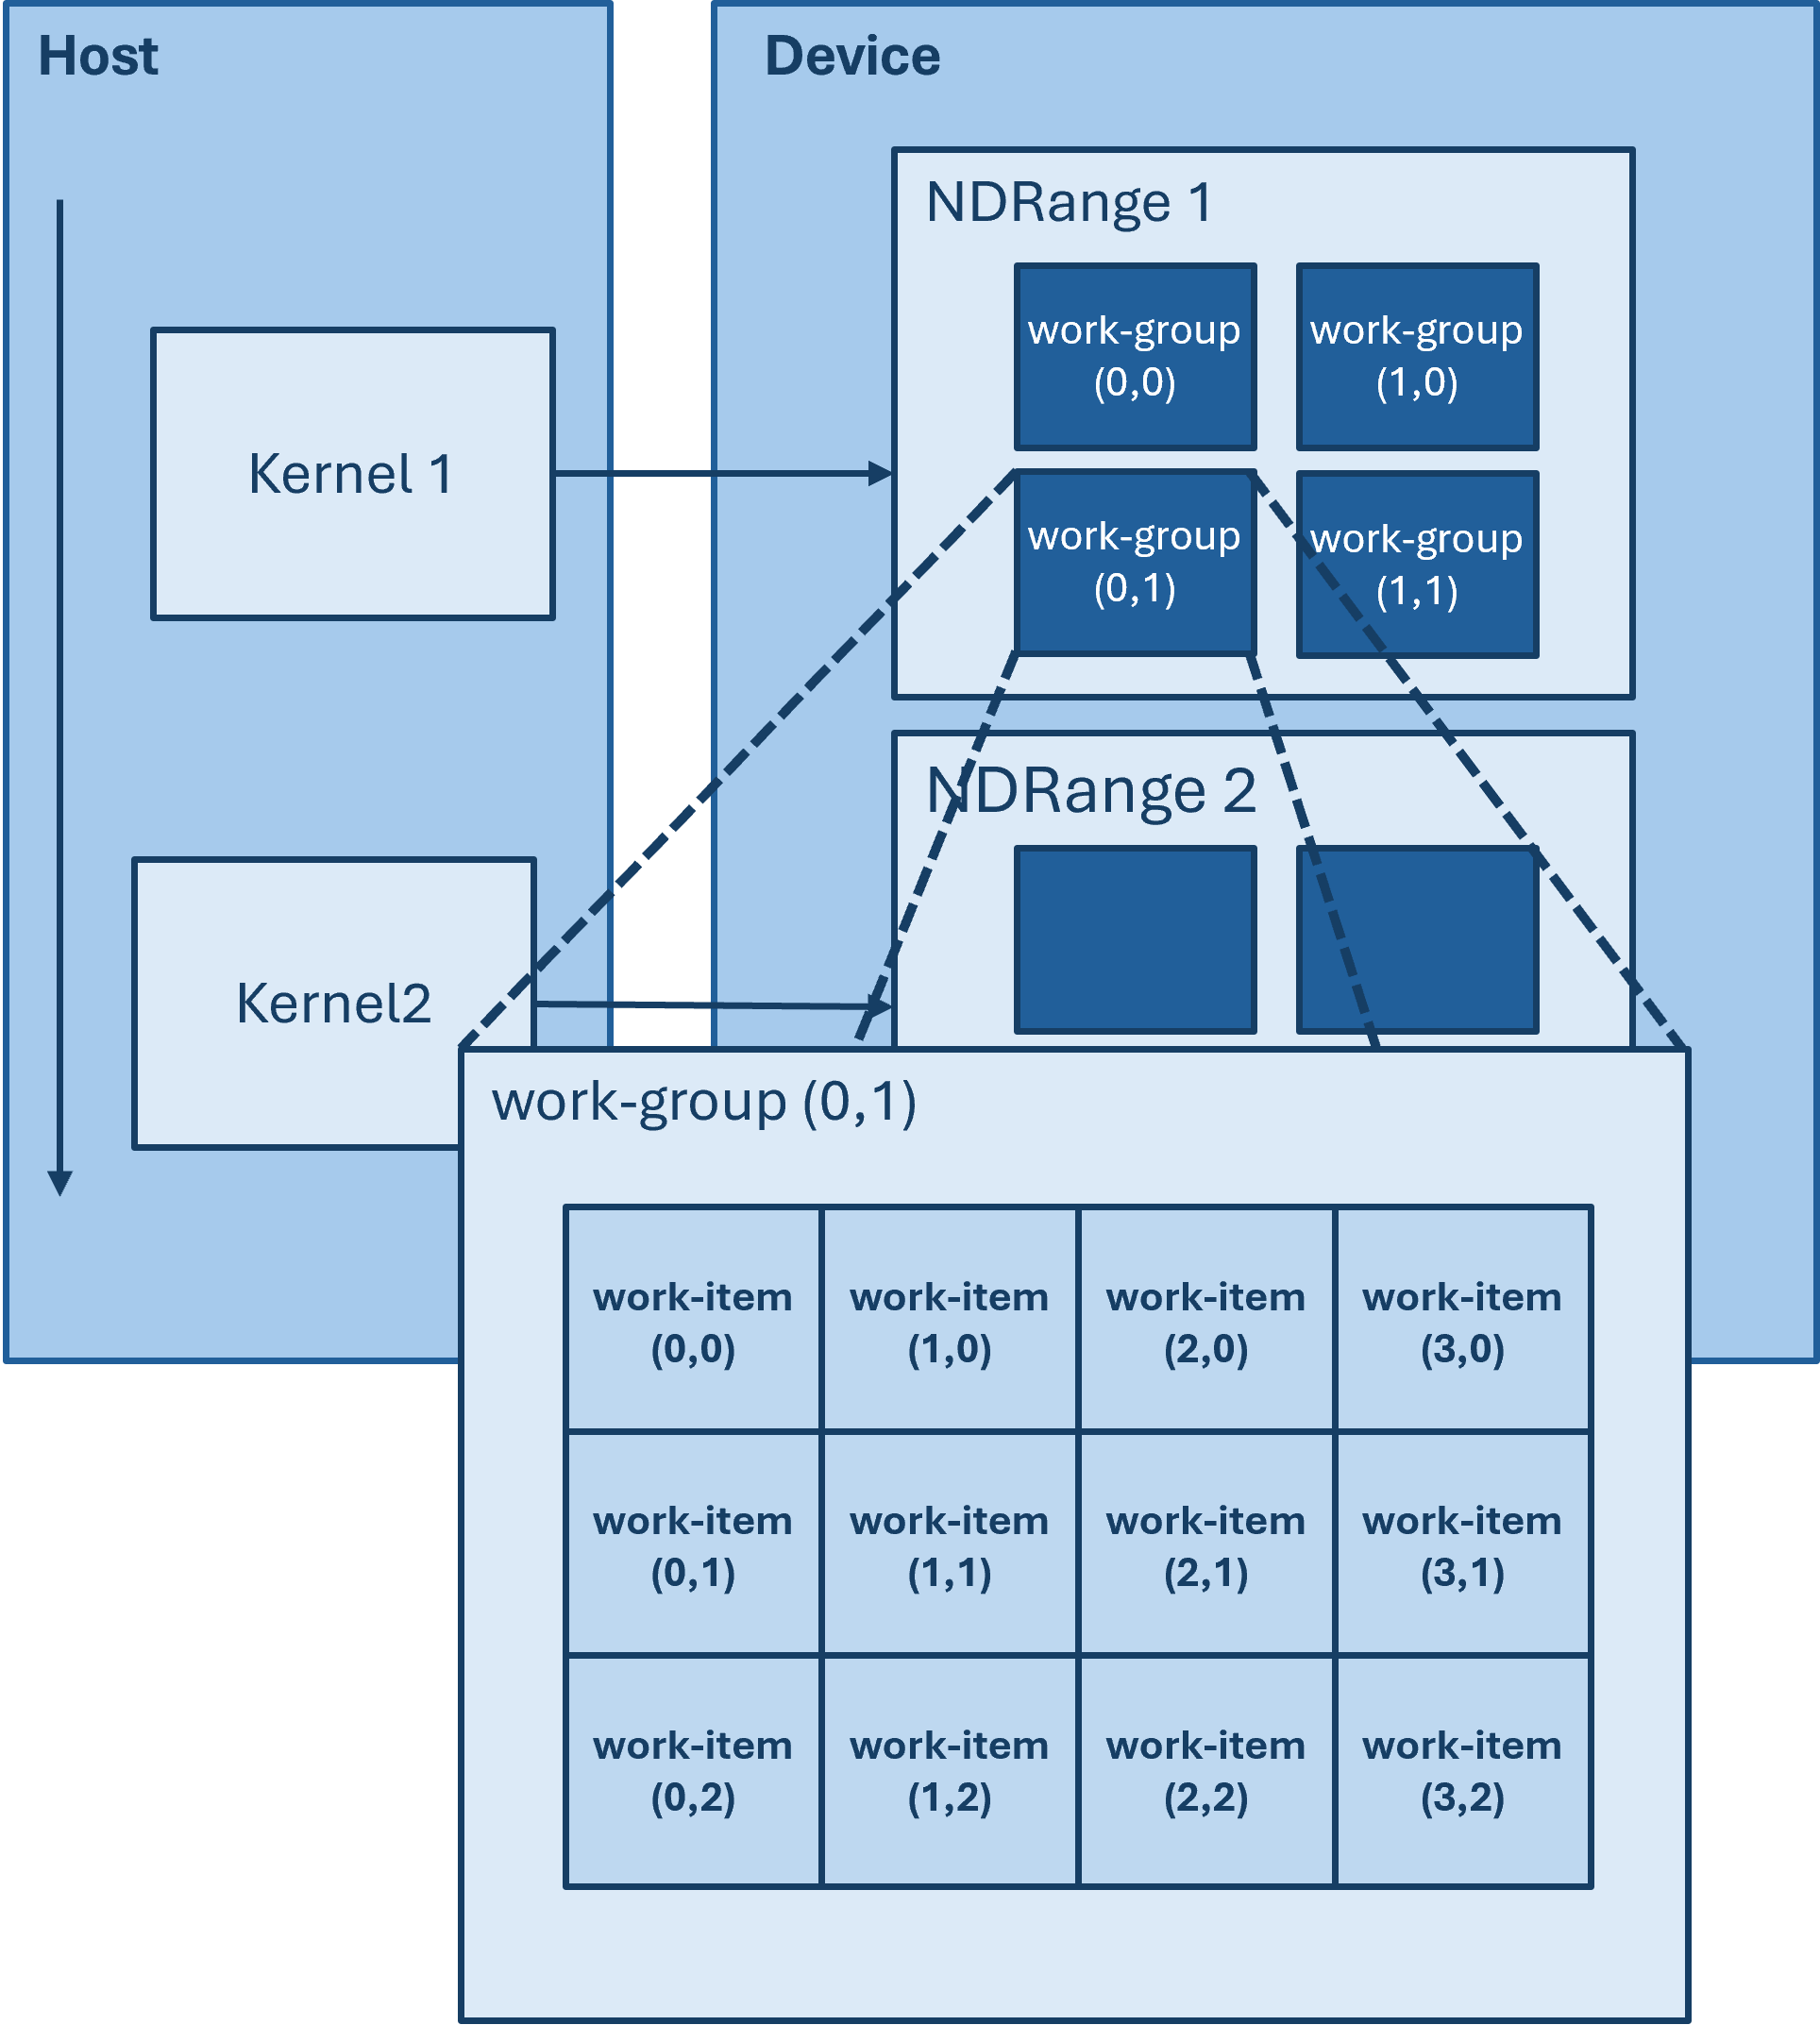
\includegraphics[width=0.6\textwidth]{img/ndrange.png}
    \caption{PISA 2-dimensional NDRange}
    \label{fig:ndrange}
\end{figure}

The virtual machine executes work-groups concurrently, but not necessarily in parallel, and the execution order 
is unspecified. Work-items of the same work-group can synchronize and communicate with each
other. Sub-groups within a work-group make independent forward progress:
unless a sub-group is waiting for another, for example at a work-group
barrier, its execution is not blocked by the other sub-groups. At the sub-group level, work-items can cooperate directly: shuffle
instructions exchange values between lanes, and reduction instructions combine
a value from every work-item into a single result~\cite{pisa-spec}.

PISA does not prescribe how the work-items of a sub-group are executed
together. Like OpenCL, its execution model is compatible with Single
Instruction, Multiple Thread (SIMT) execution, the style in which GPUs
characteristically execute work-items~\cite{lindholm-tesla}. Under SIMT,
the work-items of a sub-group execute the same instruction in lockstep, each
on its own data and registers. Lockstep execution holds only while 
every work-item in the sub-group executes the same instruction. A conditional branch can break 
that condition. If the branch predicate differs across the work-items, some take the branch and
others do not, and the sub-group \emph{diverges}. The machine cannot execute both 
paths at once, so it executes them one after another, each time executing only the 
\emph{active} work-items that belong to the path.  Work-items that do not belong to it are
\emph{inactive}: they do not participate in execution and write no results.
Divergence is confined to the sub-group, since different sub-groups execute
independently regardless of their control flow. Eventually, control flow
reaches a path common to the diverged work-items, where the inactive ones are
reactivated and rejoin execution. This is called \emph{reconvergence}. PISA does not
define a reconvergence mechanism for its virtual machine.

\subsection{Memory Model}

PISA memory is organized hierarchically into address spaces. Each work-item
has its own private memory, visible only to it, which comprises the register
and private spaces: the register space provides fast private storage, and
the private space holds memory objects private to each work-item. Each
work-group has its own shared space, in which the work-items of the
work-group may read and write any variable, synchronizing their accesses
through synchronization instructions. All work-items of an NDRange can
access the global space, which is used to exchange data with the host. A
constant space is also available as a read-only location. The parameter
space holds the kernel arguments passed from the host. It is read-only to the kernel and is written by the runtime 
before the launch. Figure~\ref{fig:memory-hierarchy} shows the spaces and the level of the work-item hierarchy
at which each becomes visible.

\begin{figure}[htbp]
    \centering
    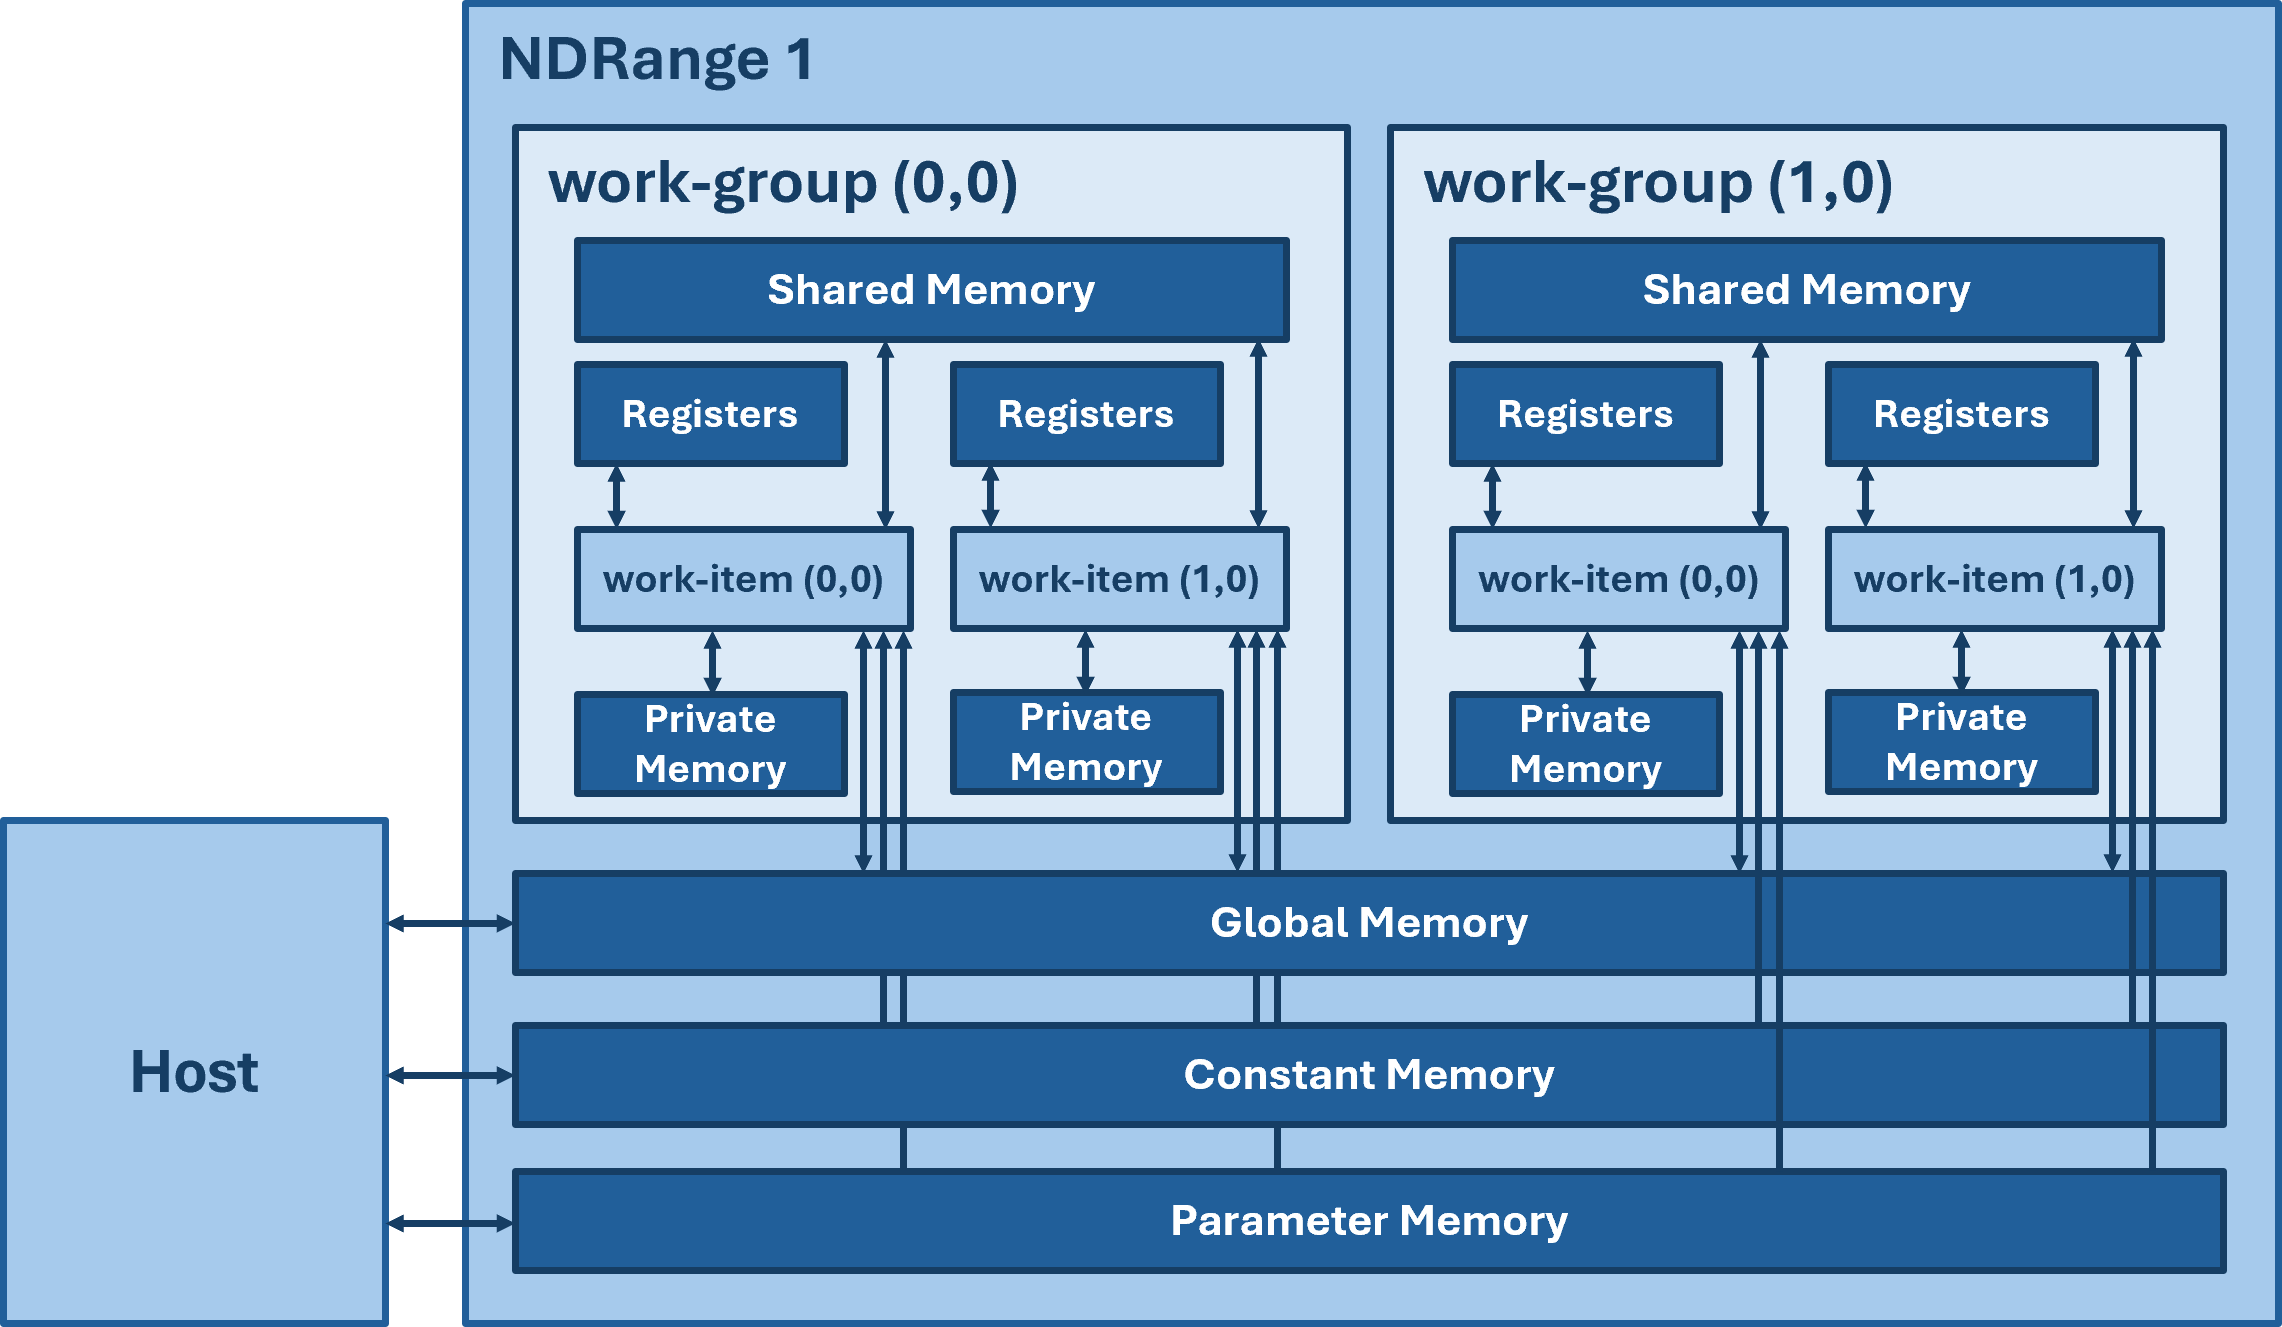
\includegraphics[width=0.6\textwidth]{img/mempisa.png}
    \caption{PISA Memory Hierarchy}
    \label{fig:memory-hierarchy}
\end{figure}

\section{The State of GPU ISA Specifications}
\label{sec:gpu-isa-state}

The GPU virtual ISAs we have presented are specified in prose. Both PTX and
PISA are documented through a natural-language reference
manual~\cite{ptx-isa, pisa-spec}. Both documents are extensive and
carefully written, but carry the risks of a prose specification, and for PTX
these risks have been measured. Lustig et al.\ constructed a formal memory
consistency model for PTX from its documentation~\cite{lustig-ptx-mcm},
and in doing so exposed ambiguities in the published text, together with
cases in which the compiler and the hardware behaved in ways no reasonable
reading of it allowed. Alglave et al.\ approached the same documentation
empirically, testing NVIDIA hardware against the behaviors the CUDA and PTX
manuals describe, and found that the hardware did not comply with its own
published specification~\cite{alglave-gpu-concurrency}. These studies
show that a prose specification can be interpreted in more than one way, and
that the implementation may differ from what has been established in prose.

Parts of GPU execution have been formalized. Habermaier and
Knapp~\cite{habermaier-simt} give a formal semantics of SIMT execution,
with lockstep, divergence, and reconvergence. They prove that a program
executed this way behaves as if its work-items were ordinary threads
interleaved one at a time. Verification tools go one level up and reason
about GPU programs directly. GPUVerify~\cite{gpuverify} takes kernels
written in OpenCL or CUDA and checks them for data races and barrier
divergence. To do so, it defines its own formal model of how a GPU executes
a kernel, encoding the execution model of those programming languages, and
verifies the kernel against it.

There are works on making PTX executable. Performance simulators such as
GPGPU-Sim and its successors~\cite{gpgpu-sim,accel-sim} run PTX
workloads on a model of the GPU microarchitecture to estimate the cost of
architectural decisions. Gutierrez et al.\ measured the cost of this abstraction: because a
virtual ISA hides the hardware by design, simulating at its level
misestimates instruction counts, register contention, and runtime by
wide margins. What a program computes, however, is the same at both
levels. The virtual ISA and the hardware ISA give it the same
semantics, and the results agree~\cite{gutierrez-lost-abstraction}.
Functional emulators work at this level and run PTX for its results alone.
Ocelot~\cite{ocelot} translates PTX for execution on CPUs and other
targets, and Claret Exojo~\cite{claret-ptx-emulation} builds an emulation
library that parses the PTX emitted by the CUDA compiler and emulates the
kernel on the CPU, reproducing the numerical results of the GPU. Both
reproduce the GPU's results from the manual alone.

Each of these lines of work delivers a piece of what a specification would
contain: the ordering of memory operations, the control-flow mechanism, an
execution model to verify programs against, and executable code that
reproduces the hardware's results. Each was built from its authors'
interpretation of the manual, and each is checked against the hardware
rather than the other way around. The same kinds of work exist for ARM,
however, all of them were carried out against one executable
specification, which served as the authority. For PTX, each was carried out
against a separate interpretation of a document. An executable specification
maintained by the ISA's provider would give these works a single reference
to start from.

\section{The Architecture Specification Language}
\label{sec:asl}

The Architecture Specification Language (ASL) is the language in which ARM
writes the pseudocode of its architecture reference manuals. The same source
renders as documentation and runs as a model. ARM publishes a formal
definition of the language, covering its type system and dynamic
semantics~\cite{asl-reference}.

ASL is an imperative language whose types are built around bitvectors of
fixed and parameterized width, alongside unbounded integers, booleans,
enumerations, records, and arrays. Architectural state is declared as
global variables, and instructions are written as functions and procedures
that read and write that state. Listing~\ref{lst:asl-add} shows a
register-to-register addition in this style.

\begin{lstlisting}[language=ASL, caption={An ASL specification of a
register-to-register addition.}, label={lst:asl-add}]
// Architectural state
var R : array[32] of bits(64);

// Instruction semantics
func ADD_reg(d : integer, n : integer, m : integer)
begin
    let operand1 = R[n];
    let operand2 = R[m];
    let result   = operand1 + operand2;
    R[d] = result;
end
\end{lstlisting}

The state is an array of 32 registers of 64 bits, and the instruction is
a procedure over it: two registers are read, added, and the result written to
a third. \lstinline{bits(64)} is a bitvector type, and the type system tracks
widths, so an expression that combines bitvectors of different widths is
rejected rather than silently coerced. A width may also be a parameter of a
function, so that one function describes an instruction for every width it
admits. Memory is provided by the built-in type \lstinline{__RAM(A)}, an
addressable store indexed by addresses of \lstinline{A} bits and read and
written in byte-sized units. A specification declares one such store per
address space it models.

Two implementations execute ASL. ASLRef is the reference implementation of
the language, developed with ARM in the herdtools7 project, whose repository
also holds the sources of the language definition~\cite{aslref}. ASLi, the
ASL interpreter, is Intel Labs' extension of ARM's original open-source
interpreter~\cite{asli}. Beyond interpreting a specification, ASLi compiles
it to C. Its \texttt{asl2c} tool takes a specification together with a
configuration file naming the functions to export, discards everything not
reachable from them, and generates C source and a supporting runtime
library. The exported functions are ordinary C functions, so a program
written in C or C\texttt{++} can initialize the specification's state, run
it, and inspect the result by calling into the generated library. ASLi's
distribution demonstrates this by building a simulator for a small example
architecture from its ASL specification, driven by a hand-written C harness.
The code generator originated in ARM's validation of its specifications,
where interpreting the specification was too slow to run the
architecture's test suites against it~\cite{reid-trustworthy-specs}.
% Capítulo: Design and Implementation
% Codificación: UTF-8

\chapter{Design and Implementation}
\label{chap:design}

The main objective of this thesis is to develop an executable specification
of PISA using ASL. The specification must be a definition of the instruction set that
can be read as its documentation and run as its reference. Specifying the
whole of PISA is beyond the scope of a thesis, so the specification covers
a subset, chosen so that the part of PISA that is distinctive of GPU
execution, the divergence and reconvergence of a sub-group, is given a
complete model of its own. This chapter presents the specification and the system built around
it to make it run.

The system has three components, shown in Figure~\ref{fig:system-overview}.
The specification, written in ASL, defines the architectural state of a
PISA sub-group and the semantics of each instruction of the subset, and
executes a kernel step by step over that state. Because PISA exists only as
text, with no binary encoding for the specification to decode, a parser
translates a PISA kernel into the ASL code that sets up the kernel's state
and instruction stream. The specification and the generated code are
compiled to C, and a host library wraps the result in an OpenCL-style
interface, so that a host program allocates buffers, launches kernels, and
reads results from the specification as it would from any OpenCL device.

\begin{figure}[t]
  \centering
  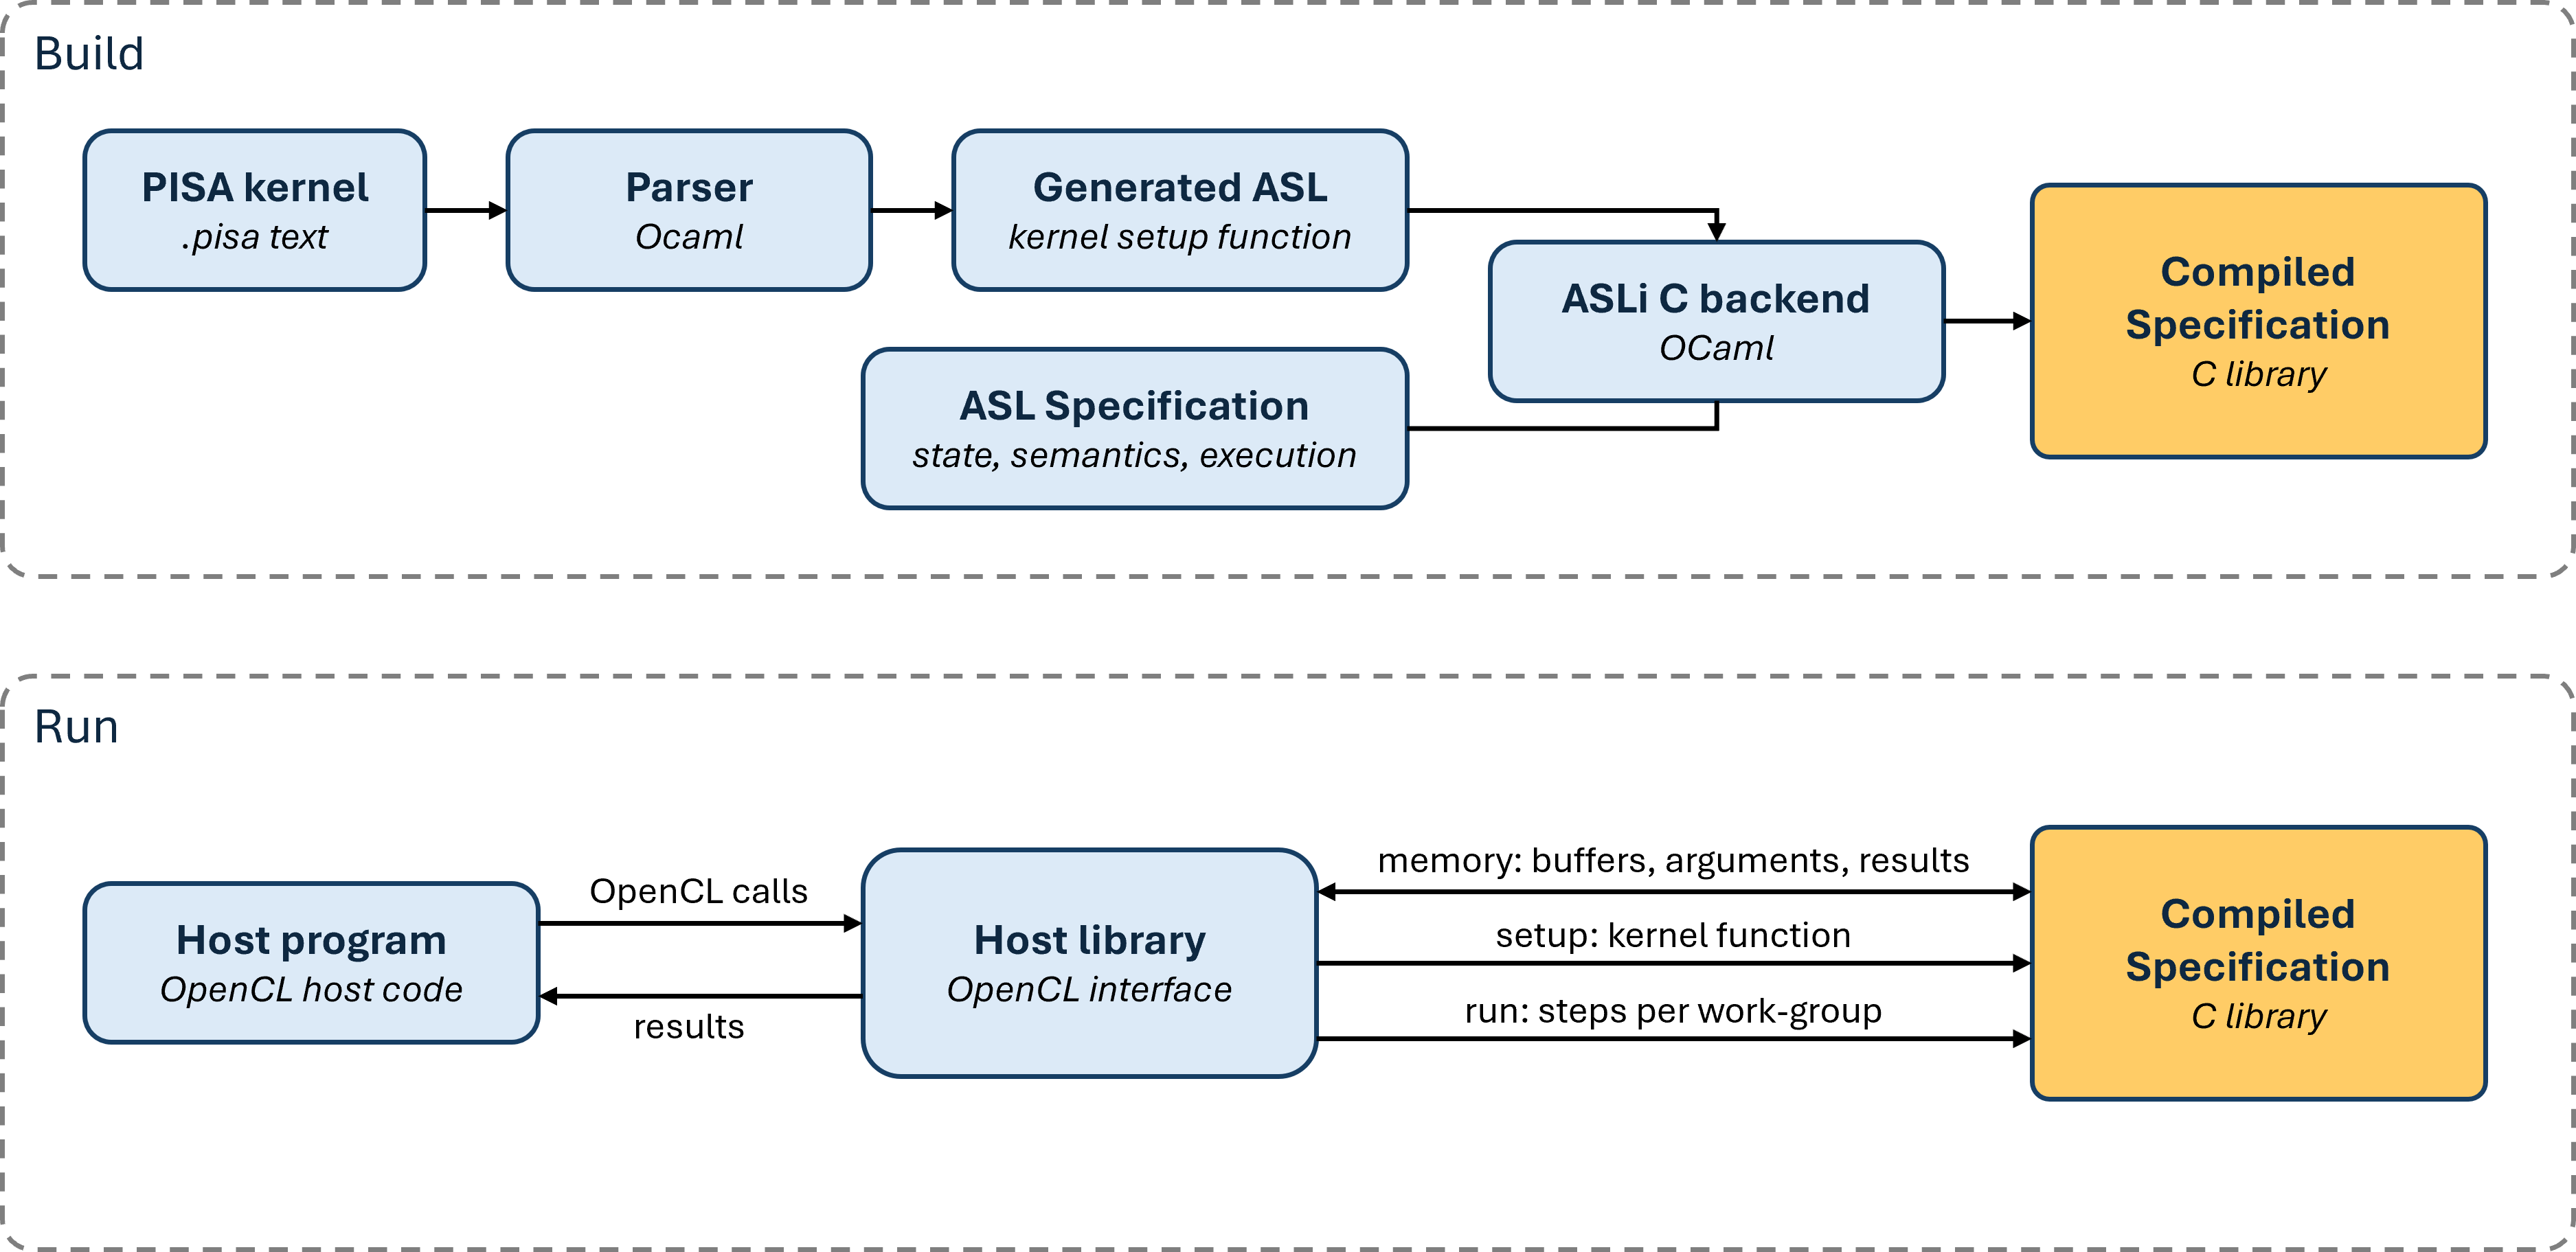
\includegraphics[width=\textwidth]{img/spec-overview.png}
  \caption[Architecture of the specification]{Architecture of the
  specification. Above, a PISA kernel is parsed into an ASL setup
  function and compiled, together with the specification, into a C
  library. Below, a host program drives that library through the OpenCL
  interface of the host library.}
  \label{fig:system-overview}
\end{figure}

The chapter follows this structure. Section~\ref{sec:pisa-subset} defines
the subset of PISA that is specified: what it contains, what it leaves out,
and the execution model it adopts. Section~\ref{sec:asl-spec} presents the
ASL specification itself: its state, its instruction semantics, the
execution model, and the handling of divergence. Section~\ref{sec:parser}
describes the parser, and Section~\ref{sec:host-library} the host library.


%--------------------------------------------------%
\section{The PISA Subset}
\label{sec:pisa-subset}

The specification covers a subset of PISA, selected so that the execution
of a sub-group can be specified completely. Throughout this document,
\emph{the subset} refers to the part of PISA defined in this section.
Within it, instruction semantics follow the published PISA specification
without modification~\cite{pisa-spec}.

Table~\ref{tab:subset-instructions} lists the instructions of the subset
by class. Every
instruction listed is supported in all of its variants.
The subset contains the instructions a kernel needs to read its inputs
from the host and write its results back, the control flow with which a
sub-group diverges and reconverges, and the instructions through which
the work-items of a sub-group communicate. It is complete enough to run
real workloads compiled from OpenCL.

\begin{table}[t]
\centering
\begin{tabular}{ll}
\toprule
Class & Instructions \\
\midrule
Logic and shift          & \texttt{and}, \texttt{or}, \texttt{xor}, \texttt{shl}, \texttt{shr}, \texttt{asr} \\
Comparison and selection & \texttt{scmp}, \texttt{ucmp}, \texttt{sel} \\
Control flow             & \texttt{goto}, \texttt{return} \\
Integer arithmetic       & \texttt{iadd}, \texttt{isub}, \texttt{smul}, \texttt{sdiv}, \texttt{udiv}, \texttt{smad}, \texttt{umad} \\
Memory                   & \texttt{ld}, \texttt{st} \\
Movement and conversion  & \texttt{mov}, \texttt{sext}, \texttt{zext}, \texttt{trunc} \\
Sub-group communication  & \texttt{shfl}, \texttt{ired} \\
\bottomrule
\end{tabular}
\caption{Instructions of the subset.}
\label{tab:subset-instructions}
\end{table}

Some major functionalities of PISA were left out of the subset to keep the
work within scope, and each omission has a cost on what the subset can do.
Floating point instructions were left out, since implementing them means
implementing the floating point logic under the IEEE rules. The cost is
that the subset cannot support any floating point workload. However, integer
arithmetic is sufficient for what this thesis wants to achieve. Function
calls were left out as well, since the specification would have to keep a call
stack per lane and reconverge lanes across calls. The cost is that the
specification cannot run a kernel whose functions a
compiler does not inline. Synchronization instructions, such as barriers, fences and atomics, were also
left out, since the specification would have to run the sub-groups of a
work-group side by side and define how they wait for one another and in
what order their memory accesses become visible. The cost is that the
specification guarantees no order of memory accesses or of instruction
execution across sub-groups, so a workload in which work-groups or
sub-groups exchange data can be racy. The remaining instructions of PISA
were left out for lack of time, or because they are newer than the
implementation of the specification. Their absence however, does not affect the
behavior of the specification. None of this is because of a limit of the specification itself,
and each omission can be added in future work.

The execution model of the subset is restricted to execution within a
sub-group. A work-group consists of one or more sub-groups of 32
work-items, so its size is a multiple of 32. A host program performs one
kernel launch, over an NDRange of such work-groups, and the model executes
the work-groups, and the sub-groups of each, one after another. Each
sub-group begins with its launch context set from the launch parameters,
which are accessible through the special registers. PISA does not define
how the work-items of a sub-group execute relative to one another. The
subset adopts lockstep execution: at each step, the active work-items
execute one instruction.


\section{The ASL Specification}
\label{sec:asl-spec}

The ASL specification is an executable model of the subset. It represents
the architectural state of one sub-group and defines, for each
instruction, how that state is transformed. A kernel runs by repeatedly
selecting the next instruction and applying its semantics to the state,
until every work-item of the sub-group has terminated.

PISA, being a virtual ISA, leaves parts of its execution open, to be
defined by each implementation that adopts it. This specification, being
an executable model, must define them as well. These definitions are
choices of the specification and are marked as such where they are made.

Section~\ref{sec:asl-state} describes the state of the model.
Section~\ref{sec:asl-instructions} describes how instruction semantics are
encoded as ASL functions. Section~\ref{sec:asl-execution} describes how
the specification executes one instruction across the sub-group, and
Section~\ref{sec:asl-divergence} how it selects the next.

\subsection{State Model}
\label{sec:asl-state}

The state of the specification is everything a sub-group's execution can
observe or modify. It falls into three groups: the memory regions that
model PISA's address spaces, the instruction buffer that holds the
program, and the execution state of each lane and of the sub-group as a
whole. Listing~\ref{lst:state-decls} shows the global declarations that
constitute it, in that order.

\begin{lstlisting}[caption={The specification's state declarations.}, label={lst:state-decls}]
// Memory: one region per address space
var RegisterSpace  : __RAM(32);
var PrivateSpace   : __RAM(32);
var SharedSpace    : __RAM(32);
var ConstantSpace  : __RAM(64);
var GlobalSpace    : __RAM(64);
var ParameterSpace : __RAM(64);

// Program
var MaxPC = 1024;
var InstructionBuffer : array[MaxPC] of Instruction;

// Execution state
var PC         : array[32] of integer;
var Done       : bits(32);
var GlobalPC   : integer;
var ActiveMask : bits(32);
\end{lstlisting}

\paragraph{Memory regions.} Each of PISA's six address spaces is a
separate \lstinline{__RAM} region, declared with an address width per
space: 32 bits for the register, private, and shared spaces, 64 bits for
the constant, global, and parameter spaces.
Separate regions apply PISA's rule that an address is interpreted within
its space: the same numeric address in two regions names two different
locations, and an instruction reaches only the region its space qualifier
names. A region has no fixed size, \lstinline{__RAM} provides the whole
address range of its width, and an address that has not been written
reads as zero.

\paragraph{Per-lane layout.} The register and private regions hold
per-work-item storage: every lane has its own copy of each register and
each private variable. A variable in these regions is therefore laid out
as 32 consecutive elements, one per lane, and a lane reaches its
element by offsetting the variable's base address by its lane index.
Figure~\ref{fig:lane-layout} shows the layout against that of a shared
variable, which exists once and is reached by every lane at the same
address. The constant, global, and parameter regions share the same layout.
Predicate registers follow the per-lane layout with one-bit elements.
Special registers are allocated in the register region and written at
kernel setup.  Some of those values can change during
execution, such as the active mask. For those their value is computed from the
execution state when read.

\begin{figure}[htbp]
    \centering
    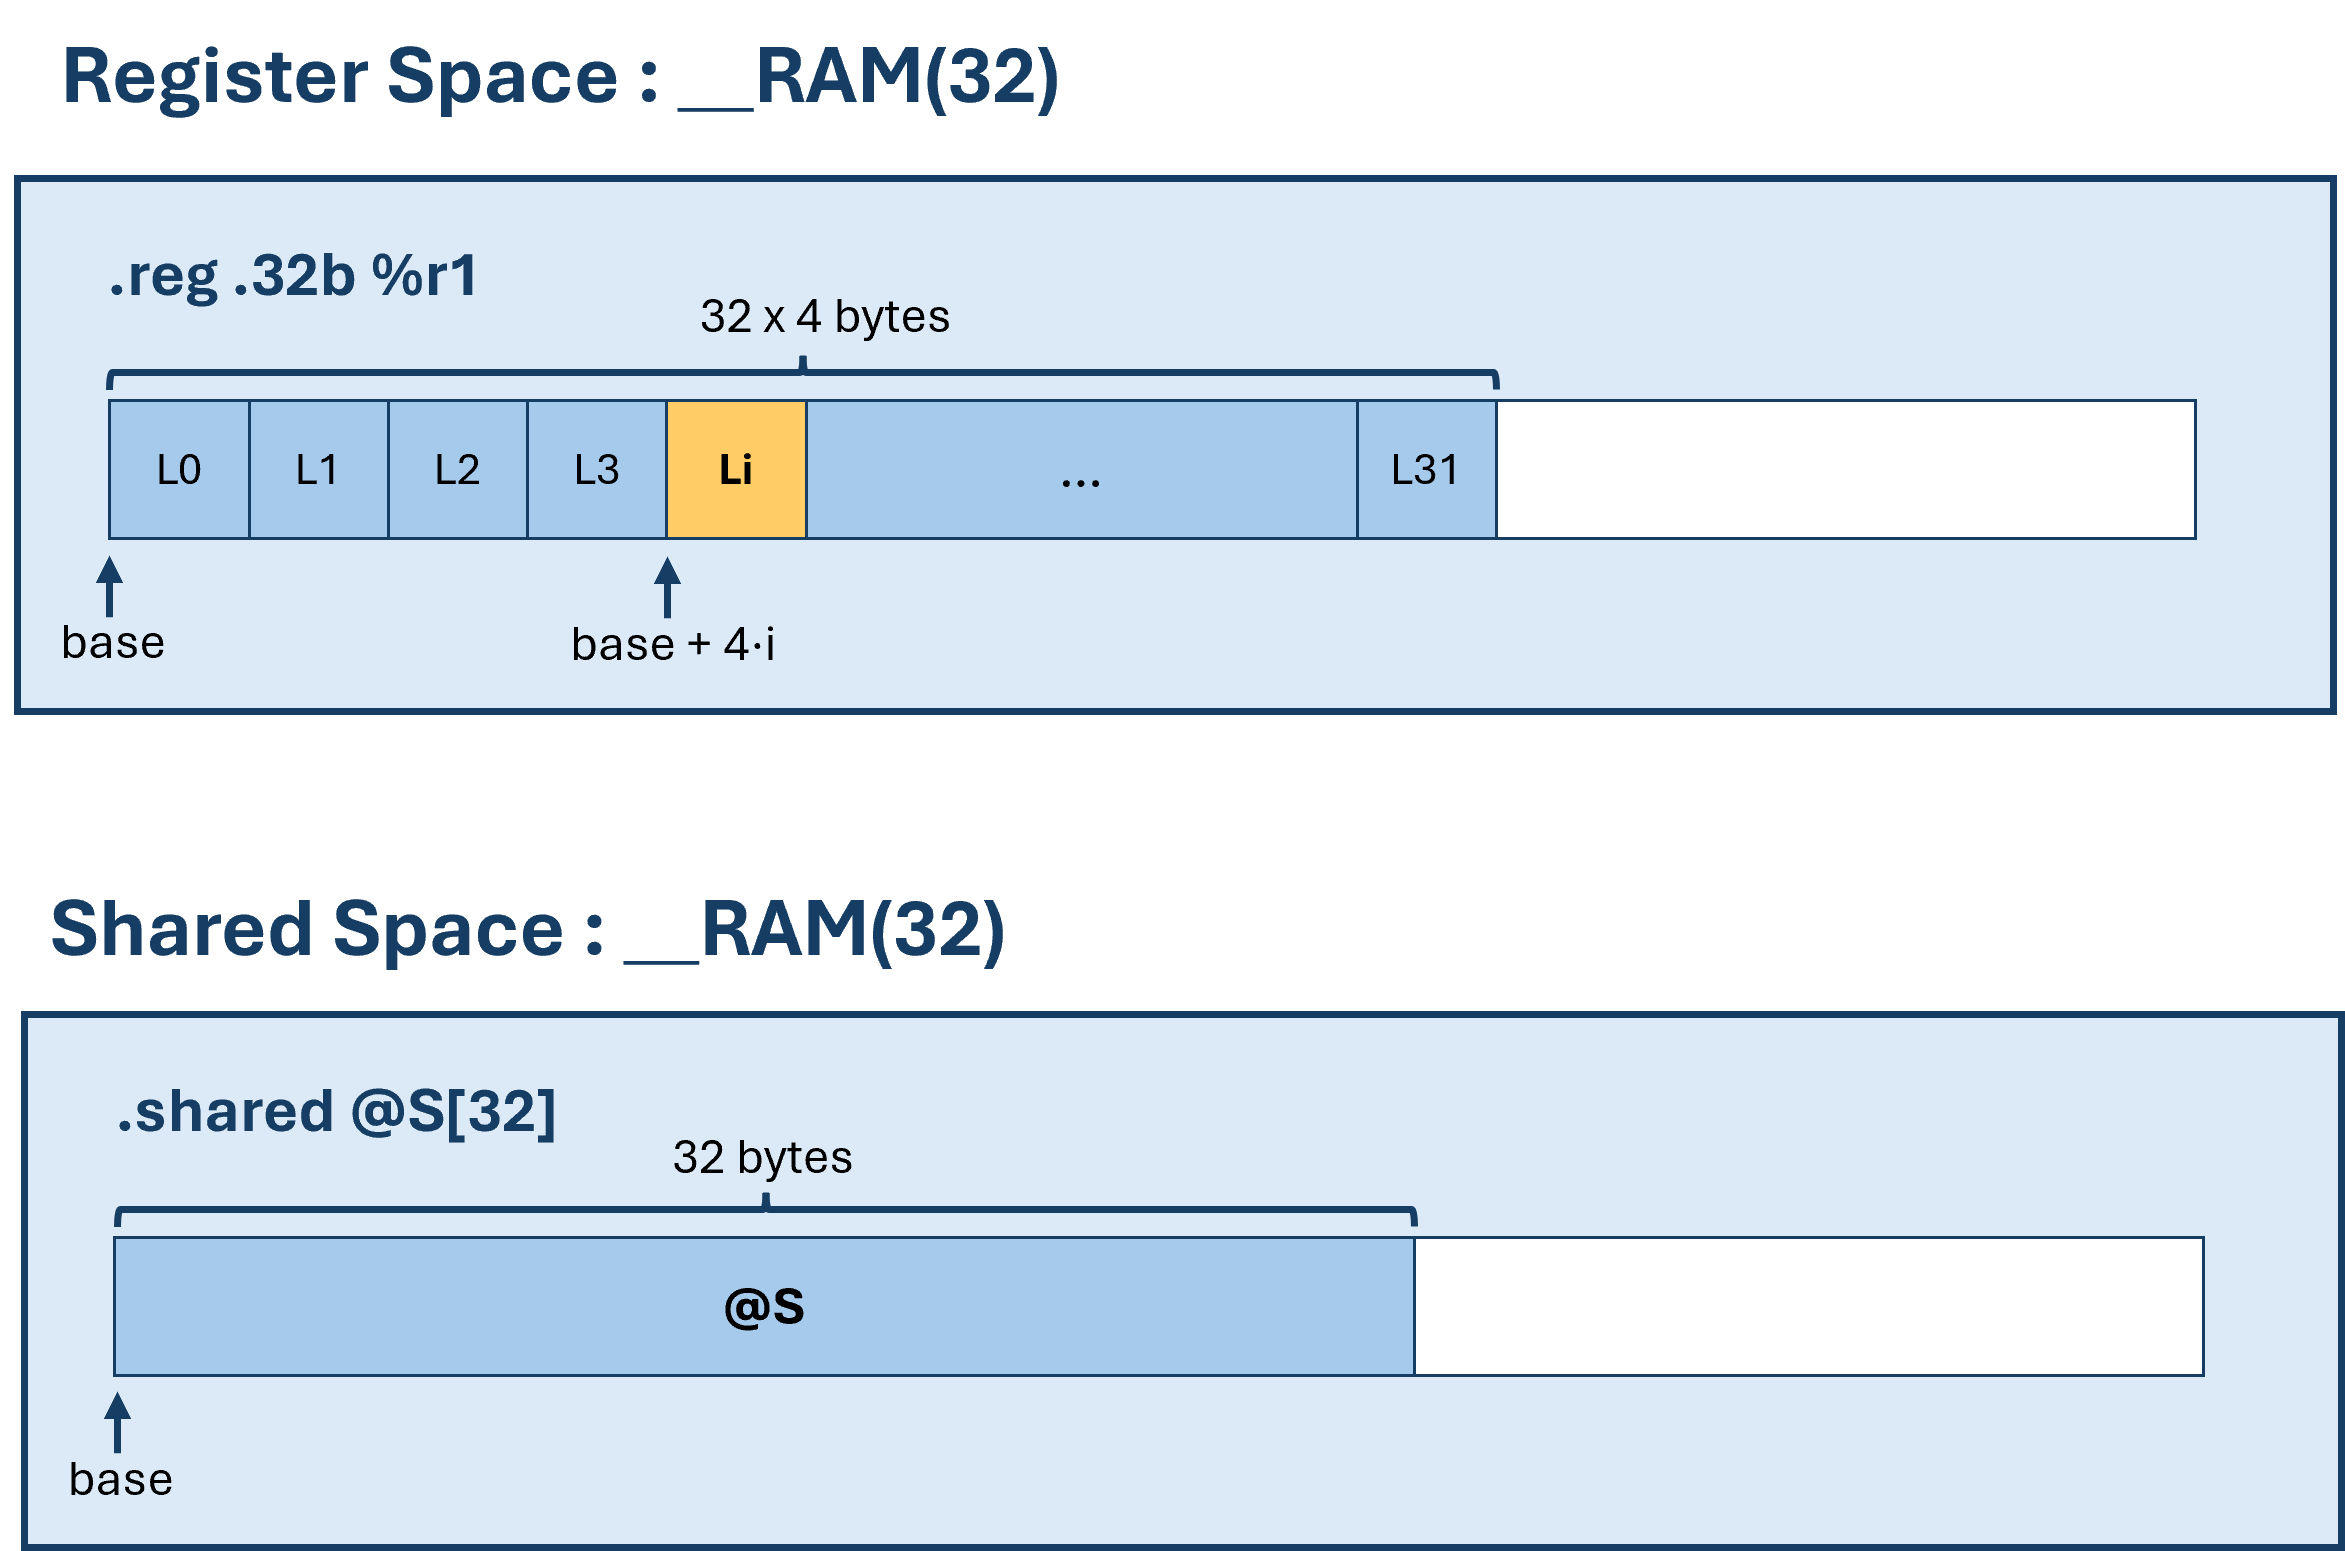
\includegraphics[width=0.85\textwidth]{img/memasl.png}
    \caption[Per-lane layout]{A register variable and a shared variable in their regions.}
    \label{fig:lane-layout}
\end{figure}

\paragraph{The variable map.} A kernel declares its variables by name, but the specification stores
them at addresses inside the memory regions, so a variable map is needed
to link the two. For every declared variable it records which region the
variable was placed in and at what address, so that an instruction that 
uses the variable as an operand can access it. It is an array of records,
Listing~\ref{lst:variable-record}, one per declared variable, holding the
variable's name, the space it lives in, its base address in that space,
its total size, and its per-lane stride. The map is also where storage is
allocated: when the setup code of a kernel declares a variable, the
specification computes its size in bytes, places it at the next free
address of its space, records the entry, and advances that space's free
pointer. The bases of Figure~\ref{fig:lane-layout} are assigned here. A
variable is identified by an integer id, assigned by the parser
(Section~\ref{sec:parser}), the emitted instructions refer to variables by
id, and the specification resolves an id to its record by searching the
array.

\begin{lstlisting}[caption={A variable-map entry.}, label={lst:variable-record}]
record Variable {
    id      : integer;        // id assigned by the parser
    name    : string;
    space   : AddressSpace;   // __RAM region
    address : bits(64);       // base address in that region
    size    : integer;        // total size in bytes
    offset  : integer;        // per-lane stride
}

var Variables : array[128] of Variable;
\end{lstlisting}


\paragraph{The program.} The kernel is held in an instruction buffer, an
array of size \lstinline{MaxPC} with one record per instruction. Listing~\ref{lst:instruction-record}
shows the record: it is wide enough to describe any instruction of the
subset, with a field for each piece of information some instruction
needs, from the opcode and operand width to the operands, immediates,
address operands, branch target, and qualifiers. Operands are represented as their ids in the
variable map, so to resolve an operand it needs to be looked up by id. The buffer is
filled by the setup code the parser generates (Section~\ref{sec:parser}),
one record per instruction of the kernel, in program order. Positions in
the buffer are the program counter values used throughout execution: a
program counter is an index into the buffer, and advancing a lane past an
instruction increments its index. Labels occupy positions of their own, as records whose opcode marks them
as labels, so a label is a program counter value like any other.

\begin{lstlisting}[caption={The instruction record (excerpt). An instruction buffer entry carries every field any instruction of the subset may need. The fields not used by an instruction are left unset.}, label={lst:instruction-record}]
record Instruction {
    opcode    : Opcode;
    bitwidth  : integer {8, 16, 32, 64};

    // operands, as variable ids
    dst       : integer;
    src0      : integer;
    src1      : integer;
    src2      : integer;
    src3      : integer;

    // immediates: flag and value per source position
    use_imm0  : boolean;
    use_imm1  : boolean;
    use_imm2  : boolean;
    use_imm3  : boolean;
    imm0      : integer;
    imm1      : integer;
    imm2      : integer;
    imm3      : integer;

    // memory access
    write_addr : boolean;
    read_addr  : boolean;
    dst_addr   : AddressOperand;
    src_addr   : AddressOperand;

    // label identifier
    label     : integer;

    // pretty print of the instruction in PISA format
    debug_string : string;

    // qualifiers
    ci        : bit;
    co        : bit;
    precision : bit;
    addrspace : AddressSpace;
    ...
}

var InstructionBuffer : array[MaxPC] of Instruction;
\end{lstlisting}

\paragraph{Execution state.} Each lane has a program counter, its
position in the instruction buffer, and a termination flag, set when the
lane executes a \texttt{return}. Because each lane has its own counter,
lanes may stand at different positions in the program, which is what
makes divergence representable. The sub-group has a global program
counter, the position of the instruction being executed in the current
step, and an active mask, one bit per lane, marking the lanes that execute
it. The \texttt{\%activemask} special
register returns this value. These values change as the kernel executes: the per-lane counters through
the control-flow instructions, and the global counter and the mask through
the specification's reconvergence mechanism.

\subsection{Instruction Semantics}
\label{sec:asl-instructions}

The semantics of each instruction of the subset are defined by an ASL
function. These functions are the executable counterpart of the
instruction's documentation in PISA: each
is the pseudocode that describes what the instruction computes, and
also the code that runs to produce that
effect. Conceptually an instruction operates on the sub-group as a whole,
one instruction applied at once across all participating lanes. Each semantic
function, however, defines the operation for one lane, and
the specification's execution model applies it across the active lanes.

For most instructions the semantic function is pure. It receives the
operand width, the instruction record, and the raw values of the source
operands, and returns the raw result, without touching the
specification's state. The reads that supply the source values and the
write that stores the result are performed by the execution model, not by
the function. A minority of instructions access state directly within
their functions: loads, branches, and the sub-group
communication instructions, since reading a memory region,
redirecting control flow, or exchanging values across lanes is the
instruction's essential effect. Keeping state accesses out of the common
case leaves each semantic function focused on the operation itself, so
that the pseudocode a reader sees expresses the instruction's behavior
without the surrounding load and store machinery, in the style of an
architecture manual. It also makes each function callable on its own,
with operands supplied directly.

Operand-width polymorphism is handled by passing the width as a
parameter. A single function serves every width variant of an instruction
by operating on the relevant slice of its operands and producing a result
of the corresponding width. Listing~\ref{lst:and_asl_impl} shows the
semantic function for the bitwise \texttt{and} instruction.

\begin{lstlisting}[caption={The semantic function of the bitwise \texttt{and} instruction. Annotated.}, label={lst:and_asl_impl}]
func and(bitwidth : integer {16, 32, 64},
         instruction : Instruction,
         src0 : bits(64),
         src1 : bits(64)) => bits(64)
begin
    var result : bits(64) = Zeros(64);

    // Extract operands at specified bit width
    let operand0 = src0[0 +: bitwidth];
    let operand1 = src1[0 +: bitwidth];

    // Perform bitwise AND operation
    let and_result = operand0 AND operand1;

    // Package result in standardized container
    result[0 +: bitwidth] = and_result;

    return result;
end
\end{lstlisting}

The function admits widths of 16, 32, or 64 bits. The source operands
arrive as 64-bit containers, of which the low \texttt{bitwidth} bits are
significant. The function extracts the operands at the requested width,
computes the result, and returns it in a container of the same form. The
instruction record is available for instructions whose behavior depends on further fields, such as a
comparison relation or a shuffle pattern. The
result is written to the instruction's destination by the execution
model.

\subsection{SIMT Execution Model}
\label{sec:asl-execution}

Execution of a kernel proceeds as a sequence of steps. At each step, the
sub-group executes the single instruction at the global program counter, on
behalf of the lanes that are currently active, and then advances. Execution
continues until every lane has terminated. This is the lockstep execution
adopted in Section~\ref{sec:pisa-subset}: at each step, one instruction is
applied across the active lanes. The specification executes each step
sequentially, visiting the active lanes one at a time, and the result is
equivalent to simultaneous execution because every read of the step happens
before any of its writes.

Every instruction that produces a value runs through a common two-pass
scheme, shown in Figure~\ref{fig:execution-step}. In the first pass, the
execution model visits each active lane in turn. For the lane, it reads
the source operands (registers at the lane's offset, special registers
from the execution state, immediates from the instruction record,
effective addresses from base and offset), calls the semantic function
selected by the opcode, and holds the result. In the second pass, it
visits the active lanes again in the same order and writes the held
results to their destinations, a register or a memory location. Because
no write happens until every lane has read, each lane's function sees the
state as it stood at the start of the step, whatever the order in which
lanes are visited. This matters when one lane's source is another lane's
destination, as in a shuffle or a reduction. \texttt{shfl} runs in the
common scheme and differs from other instructions only in reading its
source value from the selected lane's register rather than the issuing
lane's. \texttt{ired} does the same for all the active lanes at once: each
lane's function reads the contributions of every active lane and computes
the aggregate, and each lane holds and then writes its own copy. Since
the second pass writes in lane order, when several lanes write the same
memory location in one step, the value of the last lane remains.

\begin{figure}[t]
  \centering
  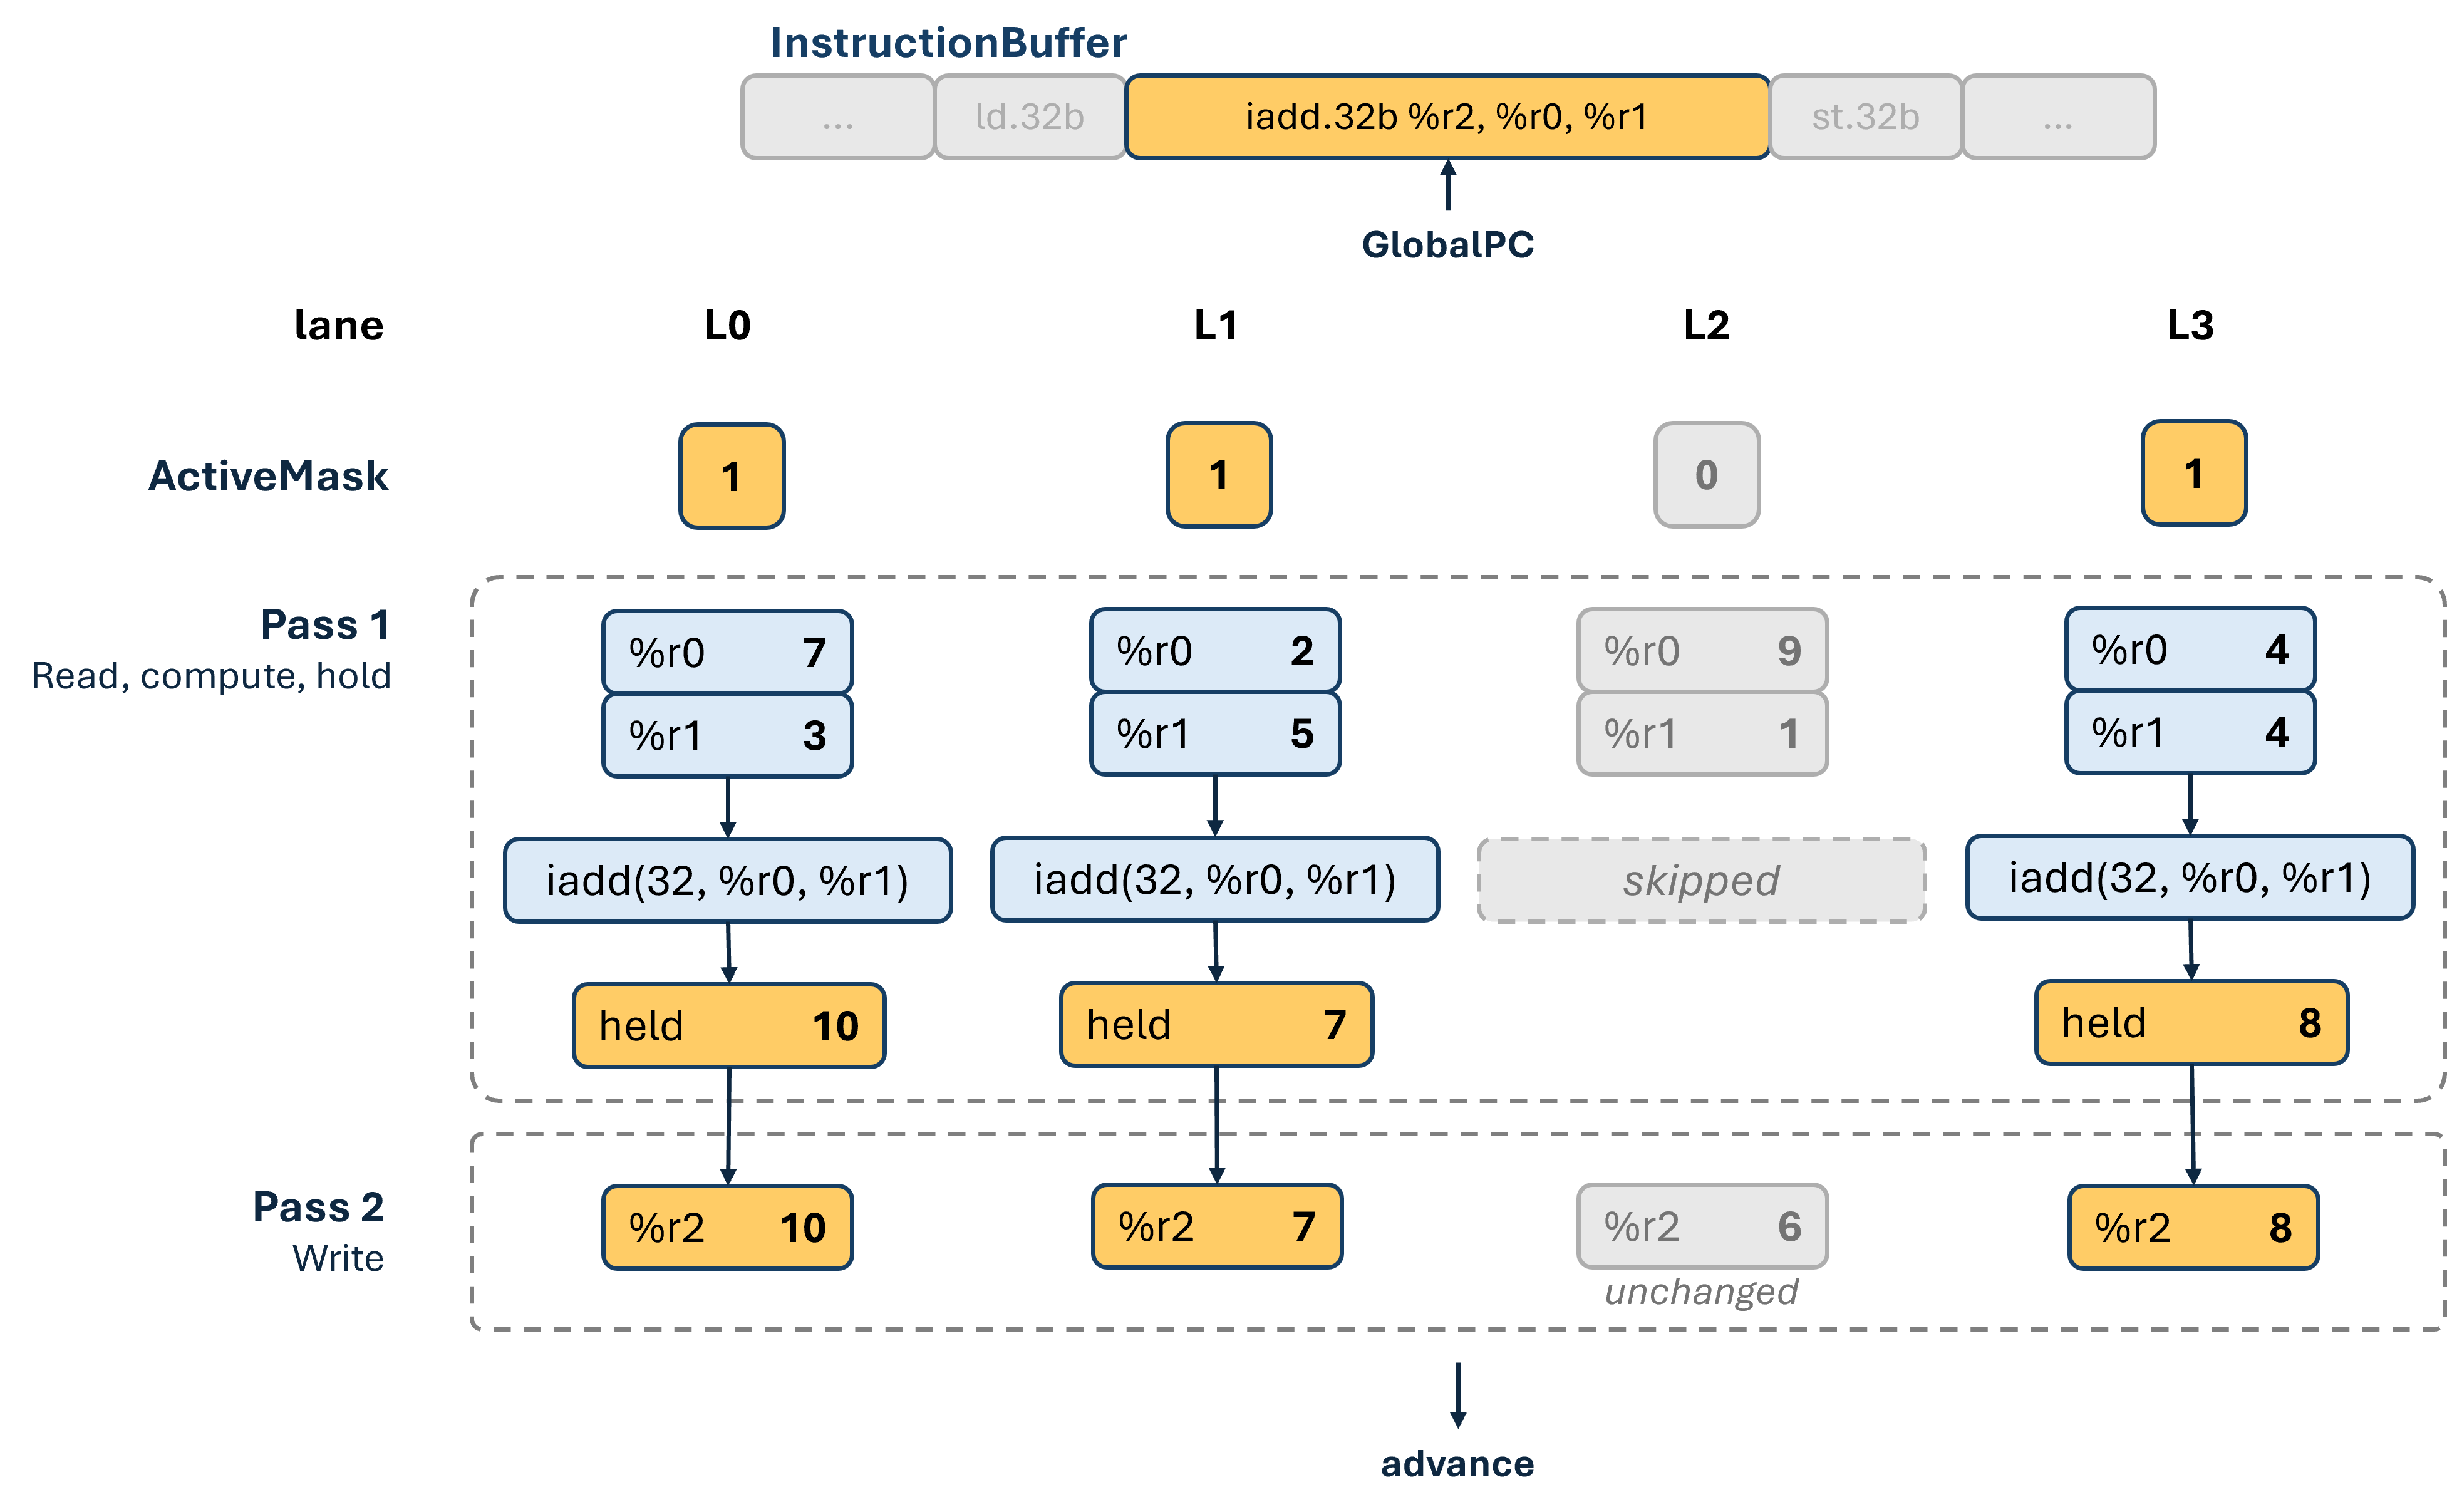
\includegraphics[width=\textwidth]{img/execution-step.png}
  \caption[One execution step]{One execution step of the common scheme.
  The instruction at the global program counter is applied to the active
  lanes: the first pass reads each lane's operands and holds the result,
  and the second pass writes the held results back. Lane 2 is inactive
  and is skipped, so its registers are unchanged.}
  \label{fig:execution-step}
\end{figure}

The \texttt{return} and \texttt{goto} instructions are the exception. They write to no
destination and only change the execution state, so they apply their
effect in the first pass: a return sets the lane's termination flag and
deactivates the lane, and a branch sets the lane's program counter. The
state they change is consulted between steps, so neither disturbs the
separation of reads and writes.

After an instruction has been executed for all active lanes, the
sub-group advances to the next step. Without divergence, every active
lane's program counter moves to the following instruction and the global
program counter advances with it. With divergence, the active lanes and
the global program counter of the next step depend on which branches the
lanes took.

\subsection{Divergence and Reconvergence}
\label{sec:asl-divergence}

The most complicated part of the execution model is its handling of
divergence. When the active lanes execute a conditional branch, they may not
all take the same direction: some will jump to the target while others fall
through, so the lanes will no longer share the same position in the program. 
Lockstep execution applies one instruction per step to all the active
lanes, so after a divergent branch, when the lanes point at different
instructions, the specification must decide which of them to run and which
will wait, and when the waiting lanes rejoin. It
must do so without reconvergence markers in the instruction stream, since
PISA exposes control flow purely as branches.

PISA defines no reconvergence mechanism, so the
specification must choose one. It resolves divergence with the implicit stackless
scheme described by Collange~\cite{collange-stackless}, which needs no
reconvergence stack and no explicit join points. This mechanism rests only on the
per-lane program counters. At the start of each step,
the global program counter is set to the minimum of the program counters
over the lanes that have not terminated, and then each lane whose counter
equals to that minimum is reactivated (Listing~\ref{lst:min-pc}). 
The instruction at the global program counter is then executed for the
active lanes. Afterwards, each active lane's counter is updated to the
next instruction, or, for a taken branch, to its target.

\begin{lstlisting}[caption={The scheduling rule, run at the start of each
step.}, label={lst:min-pc}]
func SetMinPC()
begin
    var minPC = MaxPC;
    for lane = 0 to 31 do
        if (Done[lane] == '0') && (PC[lane] < minPC) then
            minPC = PC[lane];
        end
    end
    GlobalPC = minPC;
end

func Reconverge()
begin
    for lane = 0 to 31 do
        if (Done[lane] == '0') && (ActiveMask[lane] == '0') && (PC[lane] == GlobalPC) then
            ActiveMask[lane] = '1';
        end
    end
end
\end{lstlisting}

The branch instruction does the other half of the work
(Listing~\ref{lst:goto}). A lane that executes a conditional branch sets its program
counter to the target if the predicate holds, and to the next instruction otherwise. 
For the unconditional case the branch always takes the target. The lane then marks 
itself inactive. The branch does not know whether the sub-group diverged, and it does not decide which
lanes continue: that is left to the scheduling rule at the start of the next
step. If every lane took the same direction, the rule activates them all
again and execution continues as before. If they split, the rule activates
the lanes with the lower counter and leaves the others waiting, inactive,
with their counters untouched. At each step it runs whichever lanes are
furthest behind, and when the counters coincide the lanes are active
together again. Together, the branch and the rule guarantee that, at the start of every
step, the active lanes are exactly the non-terminated lanes at the lowest
counter. Divergence and reconvergence follow from this guarantee, with no
reconvergence point recorded anywhere. The per-lane counters do the work a
reconvergence stack does in conventional implementations.

\begin{lstlisting}[caption={The semantic function of \texttt{goto}.},
label={lst:goto}]
func goto(lane : integer, pred : bit, instruction : Instruction)
begin
    let cond = instruction.goto_cond;
    let label_pc = GetLabelPC(instruction.label);
    var predicate : bit;

    if cond then
        predicate = pred;

        if instruction.flip then
            predicate = NOT predicate;
        end

        if predicate == '1' then
            PC[lane] = label_pc;
        else
            PC[lane] = GlobalPC + 1;
        end
    else
        PC[lane] = label_pc;
    end
    ActiveMask[lane] = '0';
end
\end{lstlisting}

The specification assumes that the last instruction of a kernel is a
\texttt{return}. Under this assumption no counter ever points outside the
instruction buffer: a counter moves only to
a branch target, which the parser has resolved to a slot of the buffer, or
to the next instruction, which exists for every instruction but the last,
and a lane that reaches the last instruction terminates. For a lane that
reads no value produced by another lane, execution is exactly the
sequential execution of its path: the lane runs only at its own counter,
its registers are its own, and each of its writes is complete before its
next step. Where lanes communicate, this no longer holds. A shuffle, a reduction or a
read of the mask register gives a result that depends on which lanes are
active at that step, and a value passed through memory depends on which
lane wrote it last. Both depend on the schedule.

Diverged lanes rejoin where the two paths of a branch meet again, provided
that meeting point comes after both paths in the instruction order, as it
usually does in compiler-emitted code~\cite{collange-stackless}. In other
layouts the lanes rejoin later, or elsewhere, which does not change the
results of lanes that do not communicate. A waiting lane can be starved
only by a lane behind it that never terminates. The specification places
no bound on the number of steps, so such a kernel does not complete.

Table~\ref{tab:divergence-if-else} traces the execution of a kernel with
an \texttt{if}-\texttt{else} region, over a sub-group of four lanes rather
than 32, for readability. Label slots are omitted here and in
Table~\ref{tab:divergence-loop}. The program computes a predicate that is
true for lanes~0 and~1 and false for lanes~2 and~3, branches to the
\texttt{else} block when the predicate is false, executes the
\texttt{then} block at instruction~2, branches past the \texttt{else}
block at instruction~3, executes the \texttt{else} block at
instruction~4, and reconverges at instruction~5. After the branch at
step~2, lanes~0 and~1 take the \texttt{then} path while lanes~2 and~3
wait at the \texttt{else} block. Once the \texttt{then} lanes branch past
it to instruction~5, the scheduling rule selects the waiting lanes, which
execute the \texttt{else} block and rejoin the others at step~6.

\begin{table}[h]
\centering
\begin{tabular}{c c c c l}
\toprule
Step & PCs [L0\,L1\,L2\,L3] & Global PC & Active mask & Instruction \\
\midrule
1 & 0\;0\;0\;0 & 0 & 1111 & compute predicate \\
2 & 1\;1\;1\;1 & 1 & 1111 & branch if not predicate $\to$ 4 \\
3 & 2\;2\;4\;4 & 2 & 1100 & then block \\
4 & 3\;3\;4\;4 & 3 & 1100 & branch $\to$ 5 \\
5 & 5\;5\;4\;4 & 4 & 0011 & else block \\
6 & 5\;5\;5\;5 & 5 & 1111 & end (reconverged) \\
\bottomrule
\end{tabular}
\caption{Execution trace of an \texttt{if}-\texttt{else} region.}
\label{tab:divergence-if-else}
\end{table}

Table~\ref{tab:divergence-loop} traces a loop in which lanes iterate a
different number of times: lanes~0 and~1 perform one iteration, and
lanes~2 and~3 perform two. The loop tests its condition at instruction~1,
branches out to instruction~5 when the condition fails, and returns to
the test with a backward branch at instruction~4. At step~7 the condition
fails for lanes~0 and~1, which branch to the exit and wait there. Lanes~2
and~3 remain at lower program counters and continue looping, in steps~8
to~11, until they too reach the exit, and all four lanes rejoin at
step~12.

\begin{table}[h]
\centering
\begin{tabular}{c c c c l}
\toprule
Step & PCs [L0\,L1\,L2\,L3] & Global PC & Active mask & Instruction \\
\midrule
1  & 0\;0\;0\;0 & 0 & 1111 & initialize counter \\
2  & 1\;1\;1\;1 & 1 & 1111 & test condition \\
3  & 2\;2\;2\;2 & 2 & 1111 & branch if done $\to$ 5 \\
4  & 3\;3\;3\;3 & 3 & 1111 & increment counter \\
5  & 4\;4\;4\;4 & 4 & 1111 & branch $\to$ 1 \\
6  & 1\;1\;1\;1 & 1 & 1111 & test condition \\
7  & 2\;2\;2\;2 & 2 & 1111 & branch if done $\to$ 5 \\
8  & 5\;5\;3\;3 & 3 & 0011 & increment counter \\
9  & 5\;5\;4\;4 & 4 & 0011 & branch $\to$ 1 \\
10 & 5\;5\;1\;1 & 1 & 0011 & test condition \\
11 & 5\;5\;2\;2 & 2 & 0011 & branch if done $\to$ 5 \\
12 & 5\;5\;5\;5 & 5 & 1111 & exit (reconverged) \\
\bottomrule
\end{tabular}
\caption{Execution trace of a loop with lane-dependent iteration counts.}
\label{tab:divergence-loop}
\end{table}

The two examples show the same behavior in the two directions of
branching. In the \texttt{if}-\texttt{else} region, a forward branch sends
the diverging lanes ahead, where they wait for the lanes still executing
the earlier block. In the loop, a backward branch sends the still-iterating
lanes back, where they continue while the exited lanes wait ahead. In
both, the active mask and the global program counter follow from the
per-lane program counters alone, and reconvergence happens when the
program counters coincide.

\newpage
\section{The PISA Parser}
\label{sec:parser}

A specification of a processor's instruction set, written in ASL, normally
includes a decoder: a description of how the bits of an instruction word
identify the instruction and its operands. ASL has syntax for this. However, 
PISA has no binary encoding. It exists only as text, so the
decoding step has nothing to consume.

The parser takes the place of the decoder. It accepts a kernel written in
PISA's textual syntax and produces the ASL code that, when run, sets up the
state and the instruction buffer the specification executes. It is written 
in OCaml, with ocamllex and Menhir, and runs in three
stages. The kernel text is parsed into a PISA syntax tree, which is then
transformed into a syntax tree of the ASL code to generate, and that tree
is emitted as ASL source. The output is an ASL function, specific to the kernel, that the
host library calls to set up the kernel before running it.
The parser is designed to consume the PISA text that the LLVM PISA
compiler emits~\cite{pisa-llvm-rfc}, so that compiled kernels run on the
specification without any hand editing.

\subsection{The Textual Representation}
\label{sec:parser-syntax}

The parser accepts PISA's concrete syntax~\cite{pisa-spec}, restricted to
the subset of Section~\ref{sec:pisa-subset}. A program is a single kernel:
its declaration and parameters, followed by storage declarations and a
sequence of statements, where a statement is an instruction or a label.
Listing~\ref{lst:visa-grammar} gives an excerpt of the grammar.

\begin{lstlisting}[caption={Excerpt of the accepted PISA grammar. The
address forms of memory operands are omitted.}, label={lst:visa-grammar}]
<kernel>      ::= ".kernel" "@" <identifier> "(" <params> ")"
                  "{" <declaration>* <statement>* "}"
<declaration> ::= <space> <bitwidth> <identifier>+ ";"
                | ".pred" <identifier>+ ";"
<statement>   ::= <instruction> ";" | <identifier> ":"
<instruction> ::= <opcode> <qualifier>* <operand> ("," <operand>)*
<qualifier>   ::= <bitwidth> | <space> | <condition> | ...
<space>       ::= ".reg" | ".private" | ".shared"
                | ".global" | ".const" | ".param"
<operand>     ::= <identifier> | <immediate> | "[" <address> "]"
\end{lstlisting}

An instruction is an opcode, zero or more dotted qualifiers, and a list of
operands. The qualifiers carry what the semantic functions need: the
operand width (\texttt{.32b}, \texttt{.64b}), the address space of a memory
access (\texttt{.global}, \texttt{.shared}), or the relation tested by a
comparison (\texttt{.ne}, \texttt{.lt}). Operands are registers,
immediates, or bracketed memory addresses. Declarations name the
identifiers of each address space at a given width.
Listing~\ref{lst:visa-test} shows an example kernel.

\begin{lstlisting}[caption={The \texttt{@test} kernel, a handwritten sample
with a divergent \texttt{if}-\texttt{else}.}, label={lst:visa-test}]
.kernel @test()
{
    .reg .32b %r0, %r1, %r2;
    .pred %p0;

    and.32b       %r0, %localid.x, 3;
    ucmp.ne.32b   %p0, %r0, 0;
    goto.cond     !%p0, LBB0_1;
    iadd.32b      %r1, %localid.x, -1;
    goto          LBB0_2;
LBB0_1:
    iadd.32b      %r1, %localid.x, %localid.x;
LBB0_2:
    mov.32b       %r2, %r1;
    return;
}
\end{lstlisting}

The kernel computes a predicate from the low bits of each work-item's local
identifier and branches on it, so that the two paths rejoin at
\texttt{LBB0\_2}. It has the structure of the \texttt{if}-\texttt{else}
traced in Section~\ref{sec:asl-divergence}.

\subsection{The Translation Pipeline}
\label{sec:parser-pipeline}

The first stage lexes and parses the text into a PISA syntax tree that
mirrors the grammar: a kernel node with its declarations and an ordered
list of statements. The lexer rejects malformed tokens and the parser
rejects programs outside the grammar. Beyond the grammar, the parser
assumes a well-formed kernel: every variable an instruction names is
declared, every label a branch names exists, and the last instruction
is a \texttt{return}.

The second stage transforms the PISA tree into an ASL syntax tree. Here
names become identifiers. The parser keeps a symbol table with two
namespaces, one for variables and one for labels, and assigns each name an
integer identifier when its declaration or label is first encountered. From
this point on, instructions refer to their operands and targets by
identifier.

The third stage emits ASL source from the ASL tree. Each statement takes
one slot of the instruction buffer, labels included, so the position of
every label is known once the statements are numbered. The emitted code
binds each label identifier to its slot and a branch records its label
identifier. Then the specification looks up the slot up when the branch
executes. The output is the kernel's setup function.

\subsection{Generated ASL and Kernel Setup}
\label{sec:parser-output}

The emitted function builds the kernel's state and instruction buffer
through a sequence of setup calls. It is named after the kernel
(\texttt{@test} produces \texttt{testKernel}), and the host library calls
it before running the kernel. Listing~\ref{lst:emitted-asl} shows an
excerpt of its body for \texttt{@test}.

\begin{lstlisting}[caption={Excerpt of the ASL emitted for \texttt{@test}.
Comments added for presentation.}, label={lst:emitted-asl}]
// Storage declarations: identifier, name, width
Register(0, "%r0", 32);
Register(1, "%r1", 32);
Register(2, "%r2", 32);
Pred(3, "%p0");

// Instruction encoding
InstructionBuffer[1].opcode   = ucmp;        // ucmp.ne.32b %p0, %r0, 0
InstructionBuffer[1].bitwidth = 32;
InstructionBuffer[1].cond     = ne;
InstructionBuffer[1].dst      = 3;
InstructionBuffer[1].src0     = 0;
InstructionBuffer[1].use_imm1 = TRUE;
InstructionBuffer[1].imm1     = 0;

InstructionBuffer[2].opcode    = goto;       // goto.cond !%p0, LBB0_1
InstructionBuffer[2].goto_cond = TRUE;
InstructionBuffer[2].flip      = TRUE;
InstructionBuffer[2].pred      = 3;
InstructionBuffer[2].label     = 0;
...
// Label binding: identifier, slot
SetLabel(0, 5);                              // LBB0_1
InstructionBuffer[5].opcode = label;
\end{lstlisting}

The declaration calls allocate storage when the function runs: a call such
as \texttt{Register(0, "\%r0", 32)} lays the register out across the 32
lanes of the sub-group and records its base address in the variable map.
The per-lane layout is therefore done by these calls at run time, not by
the parser. The instruction calls fill the buffer record by record, with
the opcode, qualifiers, operand identifiers and immediates that the
execution model reads. The label calls record each label's slot and mark
the slot in the buffer. Once the function has run, the state and the
instruction buffer are as the execution model expects, and the kernel can
be run.

\section{The Host Library}
\label{sec:host-library}

The ASL specification, once compiled to C, is a library of functions that
initialize the state, set up a kernel, and execute steps. The host library
wraps these functions in an interface modeled on OpenCL, so that the
specification can be used as a compute device: a host program written
against OpenCL allocates buffers, sets kernel arguments and launches
kernels on the specification as it would on any other device.

The library implements the part of OpenCL that this use needs. Allocating
buffers, transferring data to and from them, setting kernel arguments,
launching a kernel over an NDRange and reading results back are supported.
OpenCL's machinery for multiple platforms, devices, contexts and command
queues is reduced to one logical platform and one logical device, the
specification. The corresponding objects exist so that host code compiles,
but carry no configuration. Event-based synchronization and multiple
command queues are not supported, since they are not needed to run a
kernel. Two restrictions of the subset apply to every launch. Each
work-group must have a size that is a multiple of 32, which the library
enforces by rejecting any other local size. And a host program performs only
one kernel launch.

\subsection{API Surface}
\label{sec:host-api}

The library exports the OpenCL functions it supports under their standard
names, so host code written for the specification is ordinary OpenCL host
code, apart from one registration call per kernel. Listing~\ref{lst:host-usage} shows the flow of a program: it creates
a buffer, writes its input, sets the buffer as a kernel argument, launches
the kernel over an NDRange and reads the result back. The platform,
device, context and queue it refers to are created through the usual calls
and resolve to the single device the library provides.

\begin{lstlisting}[caption={Host-side usage of the library.},
label={lst:host-usage}]
size_t local_size  = 32;                 // one sub-group per work-group in this example
size_t global_size = 32 * num_groups;

cl_mem buf = clCreateBuffer(context, CL_MEM_READ_WRITE,
                            size, NULL, NULL);
clEnqueueWriteBuffer(queue, buf, CL_TRUE, 0,
                     size, input, 0, NULL, NULL);

clSetKernelArg(kernel, 0, sizeof(cl_mem), &buf);
clEnqueueNDRangeKernel(queue, kernel, 1, NULL,
                       &global_size, &local_size, 0, NULL, NULL);

clEnqueueReadBuffer(queue, buf, CL_TRUE, 0,
                    size, output, 0, NULL, NULL);
\end{lstlisting}

\subsection{Memory Mapping}
\label{sec:host-memory}

A host program communicates with a kernel through buffers, and the library
places them where PISA kernels expect them. A buffer's contents live in
global memory: creating a buffer reserves a region of the specification's
global memory, and writing to or reading from the buffer transfers the
host's data into or out of that region. Setting the buffer as a kernel
argument writes the region's address into parameter memory, at the slot of
that argument. The kernel then reads the address from parameter memory and
its loads and stores act on the region in global memory. A scalar argument
is written into parameter memory directly, so the kernel reads the value
itself from its slot.

\subsection{Kernel Launch and Execution}
\label{sec:host-launch}

A launch ties the components of this chapter together. When the host
program launches a kernel over an NDRange, the library calls the kernel's
setup function, emitted by the parser, which allocates the kernel's
variables and fills the instruction buffer. The library then runs the
work-groups of the NDRange one after another, and within each work-group
its sub-groups one after another. For each sub-group it sets the launch
context from the launch parameters, resets the rest of the state through
a function of the specification, and executes steps until every lane has
terminated. Global, constant and parameter memory persist for the whole
launch. Shared memory is reset once per work-group and persists across
its sub-groups. Registers, private memory and the execution state start
fresh for every sub-group. When the launch completes, global memory
holds the kernel's results, which the host reads back through the buffer
calls.

One part of this path is manual. A kernel is compiled into a named ASL
function rather than loaded from a binary at run time, so the library must
be told which function belongs to the kernel being launched. A host program
does this with one registration call per kernel before launching it.

% Capítulo: Evaluation
% Codificación: UTF-8

\chapter{Evaluation}
\label{chap:evaluation}

The specification is evaluated with a test suite. The suite has two
parts, each with its own reference. The smoke tests are handwritten
kernels, one per instruction, that exercise all of its variants and
compare the results with golden values derived from the PISA
document~\cite{pisa-spec}. The kernel tests run whole kernels compiled
from OpenCL and compare their outputs with an expected output computed
from the OpenCL source, by a sequential C++ program or by hand.
Every test produces a trace of the execution, step by step, which is how
the specification was debugged and where the traces shown in this
chapter come from. The suite ran after every new feature and caught the
bugs of the first versions, mainly in the handling of divergence.

As can be expected, the suite does not cover every possible case of the
subset. It is complete enough to show that execution within a sub-group
is correct: that each instruction computes what PISA prescribes, and
that kernels compose them correctly, including kernels whose work-items
diverge.

\section{Smoke Tests}
\label{sec:eval-smoke}

Since the specification was designed so that the semantics of each
instruction is a function, the smoke tests check that each of these
functions computes what the PISA document describes. There is one smoke
test per instruction, a handwritten kernel that covers every variant of
the instruction, the edge cases of its definition and the examples the
document gives.

A smoke test is a kernel with no arguments, followed by the golden values
it must produce. For each case, the kernel sets up the operands with a
few instructions, executes the subject instruction variant, and moves on to
the next case. The golden values are the expected
contents of each destination for each lane, derived from the definition
in the document. The kernel goes through the parser and runs in ASLi,
with all 32 lanes active and no host library involved. A script then
reads the values written from the trace and compares them with the
golden ones. Listing~\ref{lst:smoke-iadd} shows one case from the smoke
test of \texttt{iadd}: each lane adds $-16$ to its lane id, so lanes 0
to 15 obtain a negative result and lanes 16 to 31 a non-negative one, which
checks that the addition is signed and wraps. The suite has 26 smoke tests, 
one per instruction, with around 300 cases in all, and every case matches 
its golden values.

\begin{lstlisting}[caption={[Smoke test for iadd]Smoke
test for \texttt{iadd.32b}. The kernel is followed by the golden values
of its destination register, one per lane.}, label={lst:smoke-iadd}]
.kernel @iadd()
{
  .reg .32b %r0
  iadd.32b %r0, %laneid, -16
  return
}
GOLD
%r0 : 0xfffffff0 0xfffffff1 0xfffffff2 ... 0xd 0xe 0xf
\end{lstlisting}

When implementing \texttt{shfl}, the smoke tests made it possible to
identify two errors in the examples of the PISA
document~\cite{pisa-spec}. One was a prefix-sum example that assumed
lanes whose source is out of range do not participate, while the
actual definition says they retain their own value. The other tried to show a
segmented shuffle that moved its items down, but set its clamp value to
0, so once computed no segment was shuffled at all. Executing the
examples as written exposed both errors, and they were reported
to the PISA maintainers.

With this, the semantics of each instruction can be taken as correct.
What remains is to see how they behave together in real workloads, under
divergence, and with data that comes from a host program.


\section{Kernel Tests}
\label{sec:eval-results}

The kernel tests are built on the host library. Each test is a kernel
written in OpenCL C and compiled to PISA with a pre-release build of the
LLVM PISA compiler. Each test also has a host program that sets the
NDRange, fills the input buffers, launches the kernel through the
library, and reads the output buffer back. The expected
output of each kernel is given to the test, and the test passes when the
buffer read back matches it element by element.

The suite has 23 kernels, listed in Table~\ref{tab:suite} with their
sources in Appendix~\ref{app:kernels}, in four groups. The first group checks the basics: a kernel with no branches,
launched over one and over several work-groups, to see that arguments,
buffers and the global id reach the kernel and the results come back.
The control flow group checks that the divergence model holds from the
simple cases to the complex ones. It starts with one branch where the 
lanes split and rejoin, goes on to
nested branches and to divergent loops, and ends with two kernels that
mix loops, switches, breaks and continues into the most complex control
flow of the suite. The sub-group
communication group runs the four shuffle patterns and the sum
reduction, with all lanes active and inside divergent regions, over
one and over several sub-groups. The memory group checks that the lanes
of a work-group reach one shared
space, where a value stored by one lane can be loaded by another: each
lane stores its element and loads another lane's in a later step, with
no barrier between the two, since the subset has none. In OpenCL that is
a race. Under lockstep execution the store of one step is visible to the
load of the next, so the kernel's output is defined by the execution
model, and the exchange stays within a sub-group.

\begin{table}[t]
\centering
\small
\begin{tabular}{lp{0.55\linewidth}>{\raggedright\arraybackslash}p{0.15\linewidth}}
\toprule
Kernel & What it exercises &  Work-groups $\times$ sub-groups \\
\midrule
\multicolumn{3}{l}{\emph{Basics}} \\
\texttt{vadd}            & straight-line code, global loads and stores & 1$\times$1, 2$\times$2 \\
\midrule
\multicolumn{3}{l}{\emph{Control flow}} \\
\texttt{vadd\_if\_else}  & one divergent branch, both paths store & 1$\times$1 \\
\texttt{vadd\_mod}       & one divergent branch, half the lanes skip a region and store nothing & 1$\times$1 \\
\texttt{nested\_if}      & tree of nested divergent branches, one join before the store & 1$\times$1 \\
\texttt{loop}            & loop with lane-dependent trip count & 1$\times$2 \\
\texttt{nested\_loop}    & nested loop inside a lane-dependent loop & 1$\times$2 \\
\texttt{control\_flow}   & lane-dependent loop around a switch with fall-through, break, continue and a do-while & 1$\times$1 \\
\texttt{control\_flow1}  & as \texttt{control\_flow}, with a nested switch and an inner loop & 1$\times$1 \\
\midrule
\multicolumn{3}{l}{\emph{Sub-group communication}} \\
\texttt{shfl1}           & \texttt{shfl.idx} inside nested uniform loops, sum over lanes & 1$\times$1 \\
\texttt{shfl2}           & \texttt{shfl.idx} inside a uniform loop, broadcast of lane 31 & 1$\times$1 \\
\texttt{shfl3}           & \texttt{shfl.idx} from the next lane, index computed with \texttt{sdiv.rem} & 1$\times$1 \\
\texttt{shfl\_dn1}       & rotate-down reduction & 1$\times$1 \\
\texttt{shfl\_dn2}       & zero-fill down-reduction, unrolled, inside a uniform loop, only lane 0 stores & 1$\times$1 \\
\texttt{shfl\_dn3}       & as \texttt{shfl\_dn2}, with the reduction as a loop whose bound is computed at run time & 1$\times$1 \\
\texttt{shfl\_up1}       & rotate-up reduction, unrolled & 1$\times$1 \\
\texttt{shfl\_up2}       & rotate-up reduction, as a loop & 1$\times$1 \\
\texttt{shfl\_up3}       & zero-fill up-reduction, unrolled, inside a uniform loop, only lane 31 stores & 1$\times$1 \\
\texttt{shfl\_xor1}      & lane reversal with \texttt{shfl.xor} & 1$\times$1 \\
\texttt{shfl\_xor2}      & reversal with \texttt{shfl.xor} in a divergent region, lanes 0 to 15 only & 1$\times$1 \\
\texttt{prefix\_sum}     & inclusive scan, compiled to shuffles up & 1$\times$1, 2$\times$1 \\
\texttt{ired\_sum}       & \texttt{ired.sum} over the sub-group & 1$\times$1, 1$\times$2 \\
\texttt{reduce\_if\_else}& \texttt{ired.sum} in a divergent region, lanes 0 to 15 only & 1$\times$1, 1$\times$2 \\
\midrule
\multicolumn{3}{l}{\emph{Memory}} \\
\texttt{exchange}        & values passed between the lanes of a sub-group through shared memory, with no barrier & 2$\times$2 \\
\bottomrule
\end{tabular}
\caption[The kernel suite]{The kernel suite.}
\label{tab:suite}
\end{table}

Every kernel is launched over work-groups whose size is a multiple of
32, and the last column of Table~\ref{tab:suite} shows which kernels
also run over several work-groups or several sub-groups per work-group.
The specification records a trace of each sub-group: for every step,
the global program counter, the active mask, the instruction in PISA
syntax, and the values written. The traces in this section are
abridged to the steps that matter, and per-lane values are shown as the
pattern they follow.

Every kernel matched its expected output at every work-item, in every
launch. For a kernel without divergence, a matching output is enough.
For a divergent kernel it is not: a wrong schedule can still produce
the right output when the paths do not interact. The traces are needed
to see that the lanes diverge and reconverge as the model specifies.
The rest of this section follows four kernels through their traces: a
kernel without divergence, a kernel that diverges forward through
nested branches, a loop whose lanes leave at different times, and a
reduction under a partial mask. Masks are written with lane~0 as the
least significant bit, and a step at a label is shown by the label's
name.

\paragraph{Uniform Execution: \texttt{vadd}.}
The first kernel adds two vectors, \texttt{c[i] = a[i] + b[i]}, and has
no divergence: every work-item executes the same instructions, and the
mask is \texttt{ffffffff} at every step. It shows that the kernel as a
whole computes what its OpenCL source describes, and that data
submitted by the host reaches the kernel and comes back.

\begin{lstlisting}[language=C, caption={[Source of vadd]OpenCL source
of \texttt{vadd}.}, label={lst:src-vadd}]
__kernel void vadd(__global int *a, __global int *b, __global int *c)
{
    int i = get_global_id(0);
    c[i] = a[i] + b[i];
}
\end{lstlisting}

\begin{lstlisting}[caption={[Trace of vadd]Trace of \texttt{vadd},
abridged.}, label={lst:trace-vadd}]
PC: 0x0   mask: ffffffff   ld.param.64b %r0, [%arg0]
          %r0: 0x0 in every lane
PC: 0x1   mask: ffffffff   ld.param.64b %r1, [%arg1]
          %r1: 0x80 in every lane
PC: 0x2   mask: ffffffff   ld.param.64b %r2, [%arg2]
          %r2: 0x100 in every lane
PC: 0x3   mask: ffffffff   zext.32b.64b %r3, %localid.x
          %r3: 0, 1, 2, ..., 31
...
PC: 0x7   mask: ffffffff   asr.64b %r7, %r6, 30
          %r7: 0x0, 0x4, 0x8, ..., 0x7c
PC: 0x8   mask: ffffffff   ld.global.32b %w0, [%r0 + %r7]
          %w0: 1, 2, 3, ..., 32
PC: 0x9   mask: ffffffff   ld.global.32b %w1, [%r1 + %r7]
          %w1: 1, 2, 3, ..., 32
PC: 0xa   mask: ffffffff   iadd.32b %w2, %w1, %w0
          %w2: 2, 4, 6, ..., 64
PC: 0xb   mask: ffffffff   st.global.32b [%r2 + %r7], %w2
PC: 0xc   mask: ffffffff   return
\end{lstlisting}

Three things in the trace are worth noting. The three buffer addresses
read from parameter memory, \texttt{0x0}, \texttt{0x80} and
\texttt{0x100}, are 128 bytes apart, one buffer of 32 four-byte
elements after another, as the host library laid them out. The byte
offset in \texttt{\%r7} is four times the work-item's id, so each lane
addresses its own element. And the values stored at \texttt{0xb} run
2, 4, 6, up to 64, which is what the host reads back.

\paragraph{Forward Divergence: \texttt{nested\_if}.}
The second kernel loads one value per work-item and runs it through
nested conditionals, writing a result that depends on the path taken.
In the trace the value is the work-item's id, so the branches split the
sub-group into contiguous halves and quarters. The two innermost
levels compile to \texttt{sel}, so the kernel diverges three
times, into four groups of eight lanes, each with its own block, and
all four rejoin at one label before the store. This is the
\texttt{if}-\texttt{else} of Table~\ref{tab:divergence-if-else},
nested.

\begin{lstlisting}[caption={[Trace of nested\_if]Trace of
\texttt{nested\_if}, abridged: the three splits, the four blocks, and
the join.}, label={lst:trace-forward}]
PC: 0x5    mask: ffffffff   scmp.gt.32b %p0, %r4, 15
PC: 0x6    mask: ffffffff   goto.cond %p0, LBB0_4      ; lanes 16-31 leave
PC: 0x7    mask: 0000ffff   scmp.gt.32b %p1, %r4, 7
PC: 0x8    mask: 0000ffff   goto.cond %p1, LBB0_3      ; lanes 8-15 leave
PC: 0x9    mask: 000000ff   scmp.gt.32b %p2, %r4, 3    ; block for lanes 0-7
...
PC: 0x10   mask: 000000ff   goto LBB0_7
PC: 0x11   mask: 0000ff00   LBB0_3:                     ; lanes 8-15
...
PC: 0x18   mask: 0000ff00   goto LBB0_7
PC: 0x19   mask: ffff0000   LBB0_4:                     ; lanes 16-31
PC: 0x1a   mask: ffff0000   ucmp.gt.32b %p8, %r4, 23
PC: 0x1b   mask: ffff0000   goto.cond %p8, LBB0_6      ; lanes 24-31 leave
PC: 0x1c   mask: 00ff0000   ucmp.gt.32b %p9, %r4, 19   ; block for lanes 16-23
...
PC: 0x22   mask: 00ff0000   goto LBB0_7
PC: 0x23   mask: ff000000   LBB0_6:                     ; lanes 24-31
...
PC: 0x29   mask: ff000000   sel.16b %r8, %r13, %r14, %p12
PC: 0x2a   mask: ffffffff   LBB0_7:                     ; all rejoin
PC: 0x2b   mask: ffffffff   zext.16b.32b %r15, %r8
           %r15: 0, 0, 2, 2, 4, 4, ..., 30, 30
PC: 0x2c   mask: ffffffff   st.global.32b [%r1 + %r3], %r15
\end{lstlisting}

The point of the trace is the order of the blocks and the masks they
run under. After the splits, lanes 0 to 7 run their block alone while
lanes 8 to 15 wait at \texttt{0x11}, lanes 16 to 31 at \texttt{0x19},
and the finished lanes at the join. The lowest counter runs next, so
the four blocks execute in address order, each under the mask of its
own eight lanes, and no lane runs a block that is not its own. When
the last block reaches \texttt{0x2a}, every counter is at the join,
the mask returns to \texttt{ffffffff}, and the store executes for the
whole sub-group with each lane holding the value its own path
computed.

\paragraph{Backward Divergence: \texttt{loop}.}
The third kernel is a loop that each lane runs a different number of
times: lane $i$ runs it $i$ times and accumulates the first $i$
elements of its sub-group's block (Listing~\ref{lst:src-loop}).
Lane 0 has nothing to do and goes straight to the exit at
\texttt{LBB0\_3}, so the mask is \texttt{fffffffe} from the first
instruction after the branch. The body ends with the back-edge at
\texttt{0x13}, taken while the lane's counter is below its lane id. At
the end of every trip one lane has reached its count, falls through to
the exit, and waits there while the others go round again. The lanes
leave one per trip, in order of their id, and
Table~\ref{tab:mask-staircase} shows the mask at the back-edge on
successive trips: the cleared bits grow from the right, one per trip,
until only lane 31 remains. The only branch inside the loop is the
back-edge, so the body itself never diverges. When lane 31 falls
through, all 32 lanes are at the exit, the mask returns to
\texttt{ffffffff}, and the store runs once for every lane. The whole
kernel takes 296 steps, 31 of them back-edges. The second sub-group of
the launch produces a trace of the same shape, over its own block of
the input.

\begin{lstlisting}[language=C, caption={[Source of loop]OpenCL source
of \texttt{loop}.}, label={lst:src-loop}]
__kernel void loop(__global const int *a, __global int *out)
{
    int gid  = get_global_id(0);
    int lid  = get_sub_group_local_id();
    int base = gid - lid;
    int s = 0;
    for (int i = 0; i < lid; i++)
        s += a[base + i];
    out[gid] = s;
}
\end{lstlisting}

\begin{lstlisting}[caption={[Trace of loop]Trace of \texttt{loop},
abridged: the first back-edge, the last one, and the exit.},
label={lst:trace-loop}]
PC: 0x6   mask: ffffffff   ucmp.eq.32b %p0, %laneid, 0
PC: 0x7   mask: ffffffff   goto.cond %p0, LBB0_3
PC: 0x8   mask: fffffffe   trunc.64b.32b %w1, %d4
PC: 0x9   mask: fffffffe   isub.32b %w2, %w1, %laneid
PC: 0xa   mask: fffffffe   mov.32b %w3, %w0
PC: 0xb   mask: fffffffe   LBB0_2:
PC: 0xc   mask: fffffffe   iadd.32b %w4, %w2, %w3
PC: 0xd   mask: fffffffe   sext.32b.64b %d5, %w4
PC: 0xe   mask: fffffffe   shl.64b %d6, %d5, 2
PC: 0xf   mask: fffffffe   ld.global.32b %w5, [%d0 + %d6]
PC: 0x10  mask: fffffffe   iadd.32b %w0, %w5, %w0
PC: 0x11  mask: fffffffe   iadd.32b %w3, %w3, 1
PC: 0x12  mask: fffffffe   ucmp.lt.32b %p1, %w3, %laneid
PC: 0x13  mask: fffffffe   goto.cond %p1, LBB0_2
PC: 0xb   mask: fffffffc   LBB0_2:
...
PC: 0x13  mask: fffffffc   goto.cond %p1, LBB0_2
PC: 0xb   mask: fffffff8   LBB0_2:
...
PC: 0x13  mask: 80000000   goto.cond %p1, LBB0_2
PC: 0x14  mask: ffffffff   LBB0_3:
PC: 0x15  mask: ffffffff   shl.64b %d7, %d4, 32
PC: 0x16  mask: ffffffff   asr.64b %d8, %d7, 32
PC: 0x17  mask: ffffffff   shl.64b %d9, %d8, 2
PC: 0x18  mask: ffffffff   st.global.32b [%d1 + %d9], %w0
PC: 0x19  mask: ffffffff   return
\end{lstlisting}

In Listing~\ref{lst:trace-loop}, each omitted block is one trip of the body, from the
label at \texttt{0xb} to the back-edge, under a mask with one more bit
cleared. After the last back-edge the active lanes are exactly the
lanes at the exit label, all 32 of them.

\begin{table}[t]
\centering
\begin{tabular}{ccc}
\toprule
Trip & Mask at back-edge & Active lanes \\
\midrule
1  & \texttt{fffffffe} & 31 \\
2  & \texttt{fffffffc} & 30 \\
3  & \texttt{fffffff8} & 29 \\
\multicolumn{3}{c}{$\vdots$} \\
29 & \texttt{e0000000} & 3 \\
30 & \texttt{c0000000} & 2 \\
31 & \texttt{80000000} & 1 \\
\bottomrule
\end{tabular}
\caption[Active mask at the loop back-edge]{Active mask at the back-edge
of \texttt{loop} on successive trips.}
\label{tab:mask-staircase}
\end{table}

\paragraph{Communication under Divergence: \texttt{reduce\_if\_else}.}
The fourth kernel sums the input over the sub-group with
\texttt{ired.sum}, but only in lanes 0 to 15, which take one path of a
branch. The other 16 lanes take the other path and write $-1$
(Listing~\ref{lst:src-reduce}). The result of the reduction depends
on which lanes are active when it executes, so this is one of the
kernels on which the reconvergence model can be observed through the
output.

\begin{lstlisting}[language=C, caption={[Source of reduce\_if\_else]OpenCL
source of \texttt{reduce\_if\_else}.}, label={lst:src-reduce}]
__kernel void reduce_if_else(__global const int *a, __global int *out)
{
    int gid = get_global_id(0);
    int lid = get_sub_group_local_id();
    if (lid < 16)
        out[gid] = sub_group_reduce_add(a[gid]);
    else
        out[gid] = -1;
}
\end{lstlisting}

\begin{lstlisting}[caption={[Trace of reduce\_if\_else]Trace of
\texttt{reduce\_if\_else}, abridged: the branch, the two paths, and
the join.}, label={lst:trace-reduce}]
PC: 0x5   mask: ffffffff   ucmp.lt.32b %p0, %laneid, 16
PC: 0x8   mask: ffffffff   goto.cond %p0, LBB0_2      ; lanes 0-15 leave
PC: 0x9   mask: ffff0000   mov.32b %w0, -1            ; lanes 16-31
PC: 0xa   mask: ffff0000   goto LBB0_3
PC: 0xb   mask: 0000ffff   LBB0_2:                    ; lanes 0-15
PC: 0xc   mask: 0000ffff   ld.global.32b %w1, [%d0 + %d6]
          %w1: 1, 2, 3, ..., 16 in lanes 0-15
PC: 0xd   mask: 0000ffff   ired.sum.32b %w0, %w1, -1
          %w0: 136 in lanes 0-15, -1 in lanes 16-31
PC: 0xe   mask: ffffffff   LBB0_3:                    ; all rejoin
PC: 0xf   mask: ffffffff   st.global.32b [%d1 + %d6], %w0
PC: 0x10  mask: ffffffff   return
\end{lstlisting}

Two things in the trace (Listing~\ref{lst:trace-reduce}) matter. The
third operand of \texttt{ired.sum} is $-1$, every lane, and yet the
result is 136, the sum of 1 to 16: PISA defines the reduction over the
participating lanes that are active, and the model decides which lanes
are active at \texttt{0xd}: the 16 that took the branch. And the two paths
run in address order, lanes 16 to 31 first at \texttt{0x9} and
\texttt{0xa}, lanes 0 to 15 next at \texttt{0xb} to \texttt{0xd}, with
the join at \texttt{0xe} once every counter is there. The buffer the
host reads back holds 136 in its first 16 elements and $-1$ in
the rest, which is the expected output.

In the three divergent kernels the trace shows what the worked examples
of Section~\ref{sec:asl-divergence} showed on six instructions: the
active mask and the global program counter follow from the per-lane
counters alone, the lanes furthest behind run first, and reconvergence
happens at the step where the counters coincide, with no reconvergence
point recorded anywhere.

For 21 of the 23 kernels, the output is fixed by the instruction
semantics alone, so any correct execution of the subset must produce
it. The other two, \texttt{shfl\_xor2} and \texttt{reduce\_if\_else},
run a shuffle or a reduction under a partial mask, and their output
depends on which lanes are active at that instruction, which PISA does
not define. For these two, the expected output assumes that the lanes on the same
path reach the instruction together, as they would in a lockstep
execution of structured code. The specification produces that output,
so its reconvergence rule
activates the expected lanes.

Taken together, the smoke tests show that each instruction of the
subset computes what PISA prescribes, the kernel tests show that the
instructions compose and that the sub-group diverges and reconverges as
the model specifies.

% Capítulo: Conclusion
% Codificación: UTF-8

\chapter{Conclusion and Future Work}
\label{chap:conclusion}

The objective of this thesis was to develop an executable specification
of PISA in ASL, one that reads as documentation of the instruction set
and runs as its reference, covering a subset that models execution at
the sub-group level, with its own reconvergence model where PISA leaves
divergent control flow open, together with the tools to run kernels on
it and a test suite to check it. All of it was achieved. The
specification covers the subset of Section~\ref{sec:pisa-subset},
compiles to a C library, runs kernels compiled from OpenCL over any
number of work-groups and sub-groups, and passes every test of the
suite built to check it, against its references.

The first contribution is the specification itself. It defines the
state of a sub-group, the semantics of each instruction of the subset
as a function, and an execution model that applies one instruction per
step across the active lanes, in two passes, so that every read of a
step happens before any of its writes. Where PISA does not say how the
work-items of a sub-group execute, the specification adopts lockstep
execution, and where PISA does not say how divergent lanes reconverge,
it defines a stackless rule: at the start of every step the global
program counter is the lowest counter among the lanes that have not
terminated, and the lanes at that counter are the active ones. The rule
takes a few lines of ASL, and the active mask follows from the per-lane
program counters alone. The same source reads as a description of what
each instruction does and compiles to a library that runs it. To our
knowledge, it is the only executable specification of PISA.

The second contribution is the tooling that makes the specification
usable. PISA has no binary encoding, so a parser takes the place of a
decoder and translates a PISA kernel into the ASL function that sets up
its variables and its instruction buffer. A host library exposes the
compiled specification through the OpenCL interface, so that an
ordinary OpenCL host program allocates buffers, sets arguments,
launches a kernel over an NDRange and reads the results back. Together
they let a kernel compiled from OpenCL run on the specification without
change.

The third contribution is the test suite and the evaluation against it.
The 26 smoke tests, with around 300 cases, check every variant of every
instruction of the subset against the PISA document, and the 23 kernels
compiled from OpenCL check that the instructions compose, that the
sub-group diverges and reconverges as the model specifies, and that
data goes from the host to the kernel and back. Every case and every
kernel matches its expected output. That includes the two kernels
whose outputs depend on which lanes are active at a shuffle or a
reduction. The suite was built alongside the specification and ran
after every change. It caught the bugs of the first versions, mainly in
the handling of divergence, and it found two errors in the examples of
the PISA document, which were reported to its maintainers.

The evaluation also showed what the specification is for beyond this
thesis. The smoke tests are regression tests. If the ASL lives alongside the
PISA document, a change to an instruction is made in both, and the
tests say at once whether anything else broke. They also run the
document's own examples, which is how the two errors in them were identified.
The kernel tests also serve to check a compiler: a kernel's expected
output comes from its OpenCL source, and its actual output from the
compiled PISA run on the specification, so with the specification as
the reference, a mismatch points at the compiler. And any other tool that runs PISA kernels can be compared
with the specification by running the same kernels on the same inputs,
with no expected output needed at all.

\section{Limitations}

The specification covers a subset of PISA. It has no floating point,
no function calls, and no barriers, fences or atomics. Without floating
point it supports no floating-point workload. Without calls it cannot
run a kernel whose functions a compiler does not inline. Without
synchronization, the sub-groups of a launch run one after another, so
communication between sub-groups through memory sees the result of
that fixed order, and a workload in which sub-groups exchange data can
be racy.

PISA does not define reconvergence, so the model is a choice of the
specification, and other valid choices exist. The suite cannot tell
them apart: in the two kernels whose outputs depend on reconvergence,
the paths of every branch rejoin after both of them in instruction
order, as compiler-emitted code usually does, and on such code every common
scheme activates the same lanes at the same instructions. The rule also
orders lanes by program counter alone, which stops working once calls
are added, since a lane inside a called function can be at a lower
address than a lane that has not made the call.

Some behaviors the specification defines are not exercised by the
suite, and by design. The specification expects well-formed kernels, as
produced from real workloads by a compiler, and such kernels do not
contain unstructured branches, do not end other than in a return, and
do not store to one address from several lanes in one step. The
specification gives each of these cases a behavior, since it must do
something: it writes results back in lane order, it reconverges lanes
later or elsewhere when a join precedes a path, and it assumes that the
last instruction of a kernel is a return. It also places no bound on
the number of steps, so a kernel in which a lane never terminates does
not complete. The evaluation makes no claim about any of these cases.

The evaluation is a set of tests, so it shows that the specification
is correct on the kernels of the suite, not on every program PISA
admits. And since all the kernels were compiled with the same
pre-release build of the LLVM PISA compiler, the suite covers the code
patterns that build produces and no others.

Finally, the parser assumes a well-formed kernel, with every variable
declared and every label defined. The host
library accepts work-groups whose size is a multiple of 32 and one
kernel launch per host program.

\section{Future Work}

The first direction is extending the subset. Most of the instructions
PISA adds beyond the subset, the floating point ones first, are new
semantic functions in the existing framework and need no change to the
execution model.

The second is extending the execution model. Calls need a call stack
per lane and a reconvergence rule that accounts for call depth, since
program counter order alone no longer says which lanes are behind once
lanes are inside different calls. Collange's ordering by stack depth
before program counter~\cite{collange-stackless} is one alternative.
Barriers, fences and atomics need several sub-groups in flight at once,
with more state, a rule for scheduling between them, and a mechanism
for lanes to wait on one another. With that in place, the three have
an order to define, at the sub-group and at the work-group level.

The third is extending the test suite. Well-known test suites for GPU
algorithms, such as reductions, scans, sorting and matrix operations,
can be added once the subset supports what they need. Hand-written
PISA kernels can cover the layouts compiled code does not produce,
where the reconvergence schemes differ. And once the LLVM PISA compiler
is released upstream, the kernels of Appendix~\ref{app:kernels} can be
recompiled with it and the suite run again, to confirm that the results
hold on the released compiler.

The fourth is using the existing ASL toolchain. ASL translates into Sail, and
from Sail into emulators and into definitions for theorem
provers~\cite{isa-semantics}, where properties of the execution model
can be proved, such as the guarantee of Section~\ref{sec:asl-divergence}
that the active lanes at every step are exactly the non-terminated
lanes at the lowest counter.

The remaining directions are engineering. The parser can be completed
to accept all of PISA, so that a kernel outside the subset is reported
by the specification rather than rejected by the parser. One
observation applies here. The parser exists only because PISA has no
binary encoding. If PISA ever had one, the parser would go away: ASL
decodes instructions from their bit patterns, as the other
specifications written in it do, so the decoder would be part of the
specification itself, and supporting a new instruction would mean
adding its encoding and its semantics in one place. The host library
can accept several launches and several kernels per program, and load
kernels at run time instead of by registration. And the parts of the
specification that mirror the PISA document, the instruction tables
and the operand formats that the parser and the instruction record now
encode by hand, can be generated from the sources of the document,
which would keep the specification in step with PISA as it evolves.

\bibliographystyle{natnumurl}
\bibliography{library}

\begin{appendices}
% Apéndice: Kernel Sources
% Codificación: UTF-8

\chapter{Kernel Sources}
\label{app:kernels}

This appendix lists the OpenCL C source of every kernel of the suite of
Section~\ref{sec:eval-results}, in the order of Table~\ref{tab:suite}.
The shuffle kernels carry the \texttt{intel\_reqd\_sub\_group\_size}
attribute, which fixes the sub-group size at 32, and take the number of
elements per work-item as the argument \texttt{N}.

\section*{Basics}

\begin{lstlisting}[language=C, caption={[Source of vadd]OpenCL source of \texttt{vadd}.}, label={lst:app-vadd}]
__kernel void vadd(__global int *a, __global int *b, __global int *c)
{
    int i = get_global_id(0);
    c[i] = a[i] + b[i];
}
\end{lstlisting}

\section*{Control flow}

\begin{lstlisting}[language=C, caption={[Source of vadd\_if\_else]OpenCL source of \texttt{vadd\_if\_else}.}, label={lst:app-vadd-if-else}]
__kernel void vadd_if_else(__global int *a, __global int *b, __global int *c)
{
    int i = get_global_id(0);
    if (i % 4 == 0)
        c[i] = a[i] + b[i];
    else
        c[i] = a[i] - 1;
}
\end{lstlisting}

\begin{lstlisting}[language=C, caption={[Source of vadd\_mod]OpenCL source of \texttt{vadd\_mod}.}, label={lst:app-vadd-mod}]
__kernel void vadd_mod(__global int *a, __global int *b, __global int *c)
{
    int i = get_global_id(0);
    if (i % 2 == 0) {
        c[i + 1] = a[i + 1] + b[i];
    }
}
\end{lstlisting}

\begin{lstlisting}[language=C, caption={[Source of nested\_if]OpenCL source of \texttt{nested\_if}.}, label={lst:app-nested-if}]
__kernel void nested_if(__global int *a, __global int *b, __global int *c)
{
    int j = get_local_id(0);
    int i = a[j];
    int r = -1;
    if (i >= 16) {
        if (i >= 24) {
            if (i >= 28) {
                if (i >= 30)
                    r = 30;
                else
                    r = 28;
            }
            else if (i >= 26)
                r = 26;
            else
                r = 24;
        }
        else {
            if (i >= 20) {
                if (i >= 22)
                    r = 22;
                else
                    r = 20;
            }
            else if (i >= 18)
                r = 18;
            else
                r = 16;
        }
    }
    else {
        if (i >= 8) {
            if (i >= 12) {
                if (i >= 14)
                    r = 14;
                else
                    r = 12;
            }
            else if (i >= 10)
                r = 10;
            else
                r = 8;
        }
        else {
            if (i >= 4) {
                if (i >= 6)
                    r = 6;
                else
                    r = 4;
            }
            else if (i >= 2)
                r = 2;
            else
                r = 0;
        }
    }
    c[j] = r;
}
\end{lstlisting}

\begin{lstlisting}[language=C, caption={[Source of loop]OpenCL source of \texttt{loop}.}, label={lst:app-loop}]
__kernel void loop(__global const int *a, __global int *out)
{
    int gid  = get_global_id(0);
    int lid  = get_sub_group_local_id();
    int base = gid - lid;
    int s = 0;
    for (int i = 0; i < lid; i++)
        s += a[base + i];
    out[gid] = s;
}
\end{lstlisting}

\begin{lstlisting}[language=C, caption={[Source of nested\_loop]OpenCL source of \texttt{nested\_loop}.}, label={lst:app-nested-loop}]
__kernel void nested_loop(__global const int *a, __global int *out)
{
    int gid  = get_global_id(0);
    int lid  = get_sub_group_local_id();
    int base = gid - lid;
    int s = 0;
    __attribute__((opencl_unroll_hint(1)))
    for (int i = 0; i < lid; i++) {
        __attribute__((opencl_unroll_hint(1)))
        for (int j = 0; j < 4; j++)
            s += a[base + 4 * i + j];
    }
    out[gid] = s;
}
\end{lstlisting}

\begin{lstlisting}[language=C, caption={[Source of control\_flow]OpenCL source of \texttt{control\_flow}.}, label={lst:app-control-flow}]
__kernel void control_flow(__global int *result)
{
    int lid = get_sub_group_local_id();
    int cnt = 0;
    for (int i = 0; i < lid; i++) {
        int k = i % 8;
        switch (k) {
        case 0:
            cnt++;
            break;
        case 1:
            cnt += i;
        case 2:
            cnt--;
            break;
        case 3:
        case 4:
            cnt += 2;
            continue;
            break;
        case 5:
            {
            int j = i;
            do {
                cnt += j;
            } while (j-- > 0);
            break;
            }
        case 7:
            {
            int m = i / 8;
            if (m == 0)
                cnt--;
            else if (m == 1)
                break;
            else if (m == 2)
                continue;
            else
                cnt++;
            }
        default:
            cnt++;
        }
    }
    result[lid] = cnt;
}
\end{lstlisting}

\begin{lstlisting}[language=C, caption={[Source of control\_flow1]OpenCL source of \texttt{control\_flow1}.}, label={lst:app-control-flow1}]
__kernel void control_flow1(__global int *result)
{
    int lid = get_sub_group_local_id();
    int cnt = 0;
    for (int i = 0; i < 2 * lid; i++) {
        int k = i % 8;
        switch (k) {
        case 0:
            switch (i) {
            case 0:
                break;
            case 8:
                cnt++;
            case 16:
                continue;
                break;
            case 24:
                cnt--;
                break;
            default:
                for (int j = 0; j < i; j++) {
                    if (j < 4) {
                        cnt++;
                    }
                    else if (j == 8)
                        cnt += 3;
                    else if (j > 16 && j < 24)
                        continue;
                    else
                        cnt += 2;
                }
            }
            break;
        case 1:
            cnt += i;
        case 2:
            cnt--;
            break;
        case 3:
        case 4:
            cnt += 2;
            continue;
            break;
        case 5:
            {
            int j = i;
            do {
                cnt += j;
            } while (j-- > 0);
            break;
            }
        case 7:
            {
            int m = i / 8;
            if (m == 0)
                cnt--;
            else if (m == 1)
                break;
            else if (m == 2)
                continue;
            else
                cnt++;
            }
        default:
            cnt++;
        }
    }
    result[lid] = cnt;
}
\end{lstlisting}

\section*{Sub-group communication}

\begin{lstlisting}[language=C, caption={[Source of shfl1]OpenCL source of \texttt{shfl1}.}, label={lst:app-shfl1}]
__attribute__((intel_reqd_sub_group_size(32)))
__kernel void shfl1(__global int *a, __global int *b, __global int *c, int N)
{
    int id  = get_global_id(0);
    int lix = get_sub_group_local_id();

    int sum = 0;
    for (int i = 0; i < N; i++) {
        for (int j = 0; j < N; j++)
            sum += intel_sub_group_shuffle(a[id * N + i], j);
    }
    c[lix] = sum;
}
\end{lstlisting}

\begin{lstlisting}[language=C, caption={[Source of shfl2]OpenCL source of \texttt{shfl2}.}, label={lst:app-shfl2}]
__attribute__((intel_reqd_sub_group_size(32)))
__kernel void shfl2(__global int *a, __global int *b, __global int *c, int N)
{
    int id  = get_global_id(0);
    int lix = get_sub_group_local_id();

    int sum = 0;
    for (int i = 0; i < N; i++) {
        sum += intel_sub_group_shuffle(a[id * N + i], 31);
    }
    c[lix] = sum;
}
\end{lstlisting}

\begin{lstlisting}[language=C, caption={[Source of shfl3]OpenCL source of \texttt{shfl3}.}, label={lst:app-shfl3}]
__attribute__((intel_reqd_sub_group_size(32)))
__kernel void shfl3(__global int *a, __global int *b, __global int *c, int N)
{
    int id = get_global_id(0);

    int sum = 0;
    for (int i = 0; i < N; i++) {
        int lix = (id + 1) % 32;
        sum += intel_sub_group_shuffle(a[id * N + i], lix)
             * intel_sub_group_shuffle(b[id * N + i], lix);
    }
    c[id] = sum;
}
\end{lstlisting}

\begin{lstlisting}[language=C, caption={[Source of shfl\_dn1]OpenCL source of \texttt{shfl\_dn1}.}, label={lst:app-shfl-dn1}]
__attribute__((intel_reqd_sub_group_size(32)))
__kernel void shfl_dn1(__global int *a, __global int *b, __global int *c, int N)
{
    int id  = get_global_id(0);
    int lix = get_sub_group_local_id();

    int red = a[id * N] * b[id * N];

    for (int j = 16; j > 0; j = j / 2)
        red += intel_sub_group_shuffle_down(red, red, j);
    c[lix] = red;
}
\end{lstlisting}

\begin{lstlisting}[language=C, caption={[Source of shfl\_dn2]OpenCL source of \texttt{shfl\_dn2}.}, label={lst:app-shfl-dn2}]
__attribute__((intel_reqd_sub_group_size(32)))
__kernel void shfl_dn2(__global int *a, __global int *b, __global int *c, int N)
{
    int id  = get_global_id(0);
    int lix = get_sub_group_local_id();

    for (int i = 0; i < N; i++) {
        int red = a[id * N + i] * b[id * N + i];

        for (int j = 16; j > 0; j = j / 2)
            red += intel_sub_group_shuffle_down(red, 0, j);
        if (lix == 0)
            c[i] = red;
    }
}
\end{lstlisting}

\begin{lstlisting}[language=C, caption={[Source of shfl\_dn3]OpenCL source of \texttt{shfl\_dn3}.}, label={lst:app-shfl-dn3}]
__attribute__((intel_reqd_sub_group_size(32)))
__kernel void shfl_dn3(__global int *a, __global int *b, __global int *c, int N)
{
    int id  = get_global_id(0);
    int lix = get_sub_group_local_id();

    for (int i = 0; i < N; i++) {
        int red = a[id * N + i] * b[id * N + i];

        for (int j = N / 2; j > 0; j = j / 2)
            red += intel_sub_group_shuffle_down(red, 0, j);
        if (lix == 0)
            c[i] = red;
    }
}
\end{lstlisting}

\begin{lstlisting}[language=C, caption={[Source of shfl\_up1]OpenCL source of \texttt{shfl\_up1}.}, label={lst:app-shfl-up1}]
__attribute__((intel_reqd_sub_group_size(32)))
__kernel void shfl_up1(__global int *a, __global int *b, __global int *c, int N)
{
    int id  = get_global_id(0);
    int lix = get_sub_group_local_id();

    int red = a[id * N] * b[id * N];

    for (int j = 16; j > 0; j = j / 2)
        red += intel_sub_group_shuffle_up(red, red, j);
    c[lix] = red;
}
\end{lstlisting}

\begin{lstlisting}[language=C, caption={[Source of shfl\_up2]OpenCL source of \texttt{shfl\_up2}.}, label={lst:app-shfl-up2}]
__attribute__((intel_reqd_sub_group_size(32)))
__kernel void shfl_up2(__global int *a, __global int *b, __global int *c, int N)
{
    int id  = get_global_id(0);
    int lix = get_sub_group_local_id();

    int red = a[id * N] * b[id * N];

    for (int j = N / 2; j > 0; j = j / 2)
        red += intel_sub_group_shuffle_up(red, red, j);
    c[lix] = red;
}
\end{lstlisting}

\begin{lstlisting}[language=C, caption={[Source of shfl\_up3]OpenCL source of \texttt{shfl\_up3}.}, label={lst:app-shfl-up3}]
__attribute__((intel_reqd_sub_group_size(32)))
__kernel void shfl_up3(__global int *a, __global int *b, __global int *c, int N)
{
    int id  = get_global_id(0);
    int lix = get_sub_group_local_id();

    for (int i = 0; i < N; i++) {
        int red = a[id * N + i] * b[id * N + i];

        for (int j = 16; j > 0; j = j / 2)
            red += intel_sub_group_shuffle_up(0, red, j);
        if (lix == 31)
            c[i] = red;
    }
}
\end{lstlisting}

\begin{lstlisting}[language=C, caption={[Source of shfl\_xor1]OpenCL source of \texttt{shfl\_xor1}.}, label={lst:app-shfl-xor1}]
__attribute__((intel_reqd_sub_group_size(32)))
__kernel void shfl_xor1(__global int *a, __global int *b, __global int *c, int N)
{
    int id  = get_global_id(0);
    int lix = get_sub_group_local_id();

    int sum = 0;
    for (int i = 0; i < N; i++) {
        sum += intel_sub_group_shuffle_xor(a[id * N + i], 0x1F)
             * intel_sub_group_shuffle_xor(b[id * N + i], 0x1F);
    }
    c[lix] = sum;
}
\end{lstlisting}

\begin{lstlisting}[language=C, caption={[Source of shfl\_xor2]OpenCL source of \texttt{shfl\_xor2}.}, label={lst:app-shfl-xor2}]
__attribute__((intel_reqd_sub_group_size(32)))
__kernel void shfl_xor2(__global int *a, __global int *b, __global int *c, int N)
{
    int id  = get_global_id(0);
    int lix = get_sub_group_local_id();

    if (lix < 16) {
        int sum = 0;
        for (int i = 0; i < N; i++) {
            sum += intel_sub_group_shuffle_xor(a[id * N + i], 0xF)
                 * intel_sub_group_shuffle_xor(b[id * N + i], 0xF);
        }
        c[lix] = sum;
    }
}
\end{lstlisting}

\begin{lstlisting}[language=C, caption={[Source of prefix\_sum]OpenCL source of \texttt{prefix\_sum}.}, label={lst:app-prefix-sum}]
__kernel void prefix_sum(__global const int *a, __global int *b)
{
    uint gid = get_global_id(0);
    int x = a[gid];

    b[gid] = sub_group_scan_inclusive_add(x);
}
\end{lstlisting}

\begin{lstlisting}[language=C, caption={[Source of ired\_sum]OpenCL source of \texttt{ired\_sum}.}, label={lst:app-ired-sum}]
__kernel void ired_sum(__global int *a, __global int *c)
{
    int id = get_global_id(0);
    c[id] = sub_group_reduce_add(a[id]);
}
\end{lstlisting}

\begin{lstlisting}[language=C, caption={[Source of reduce\_if\_else]OpenCL source of \texttt{reduce\_if\_else}.}, label={lst:app-reduce-if-else}]
__kernel void reduce_if_else(__global const int *a, __global int *out)
{
    int gid = get_global_id(0);
    int lid = get_sub_group_local_id();
    if (lid < 16)
        out[gid] = sub_group_reduce_add(a[gid]);
    else
        out[gid] = -1;
}
\end{lstlisting}

\section*{Memory}

\begin{lstlisting}[language=C, caption={[Source of exchange]OpenCL source of \texttt{exchange}.}, label={lst:app-exchange}]
__kernel void exchange(__global const int *a, __global int *out)
{
    __local int buf[32];
    int gid = get_global_id(0);
    int lid = get_sub_group_local_id();
    buf[lid] = a[gid];
    out[gid] = buf[31 - lid];
}
\end{lstlisting}
\end{appendices}

\end{document}
